%------------------------------------------%
% Cannabis Data Science
% Date: 1/4/2024
%------------------------------------------%
\documentclass[xcolor={dvipsnames}]{beamer}
\hypersetup{pdfpagemode = FullScreen}
\mode<presentation>{
  \usetheme{Boadilla}
  \usecolortheme{orchid}
  \usefonttheme{default}
  \setbeamertemplate{navigation symbols}{}
  \setbeamertemplate{caption}[numbered]
}
\setbeamersize{
  text margin left = 0.5in,
  text margin right = 0.5in
}

%------------------------------------------%
% Title
%------------------------------------------%
\title[\textbf{Cananbis Data Science \#141}]{}
\author{Cannabis Data Science}
\institute[]{\Large Cananbis Data Science \#141}
\date{January \nth{4}, 2024}

%------------------------------------------%
% Packages
%------------------------------------------%
\usepackage[english]{babel}
\usepackage[utf8x]{inputenc}
\usepackage{tikz}
\usepackage{xparse}

%------------------------------------------%
% Colors
%------------------------------------------%
\definecolor{Green}{RGB}{34, 153, 84}
\definecolor{LightGreen}{RGB}{218, 247, 166}
\definecolor{DarkGreen}{RGB}{2, 48, 32}
\definecolor{Orange}{RGB}{255, 87, 51}
\definecolor{DarkOrange}{RGB}{199, 0, 57}
\definecolor{Yellow}{RGB}{255, 195, 0}

%------------------------------------------%
% Theme
%------------------------------------------%
\setbeamercolor*{palette primary}{bg=LightGreen, fg=DarkGreen}
\setbeamercolor*{palette secondary}{bg=LightGreen, fg=DarkGreen}
\setbeamercolor*{palette tertiary}{bg=LightGreen, fg=DarkGreen}

%------------------------------------------%
% Packages
%------------------------------------------%
\usepackage{amsmath}
\renewcommand*\footnoterule{}
\usepackage{mathtools}
\usepackage{hhline}
\usepackage[super]{nth}
\usepackage{graphicx, caption, subcaption}

%------------------------------------------%
% Commands
%------------------------------------------%

% Top space.
\newcommand\T{\rule{0pt}{2.5ex}}

% Bottom space.
\newcommand\B{\rule[-1.25ex]{0pt}{0pt}}

% Blocks.
\newenvironment<>{Block}[2][.9\textwidth]
  {\setlength{\textwidth}{#1}
  \begin{actionenv}#3
    \def\insertblocktitle{#2}\par
    \usebeamertemplate{block begin}}
  {\par\usebeamertemplate{block end}
  \end{actionenv}}

% Balls.
\defbeamertemplate{enumerate item}{largeball}
{\begin{pgfpicture}{-1ex}{-0.65ex}{1.5ex}{1.5ex}
\usebeamercolor[fg]{item projected}
{\pgftransformscale{2.5}\pgftext{\Large\pgfuseshading{bigsphere}}}
{\pgftransformshift{\pgfpoint{0pt}{0.5pt}}
\pgftext{\usebeamerfont*{item projected}\small\insertenumlabel}}
\end{pgfpicture}}

% Fancy arrows.
\NewDocumentCommand\UpArrow{O{2.0ex} O{black}}{%
   \mathrel{\tikz[baseline] \draw [->, line width=0.5pt, #2] (0,0) -- ++(0,#1);}} % Fancy up-arrow.
\NewDocumentCommand\DownArrow{O{2.0ex} O{black}}{%
   \mathrel{\tikz[baseline] \draw [<-, line width=0.5pt, #2] (0,0) -- ++(0,#1);}} % Fancy down-arrow.

% Equations with numbers on the left.
\makeatletter
\newcommand{\LeftEqNo}{\let\veqno\@@leqno}
\makeatother

%------------------------------------------%
% Presentation
%------------------------------------------%
\begin{document}

% Title page.
\begin{frame}{}
  
\includegraphics[scale=0.33]{images/logo.pdf}
  \vspace*{-2\baselineskip}
  \titlepage
\end{frame}

%------------------------------------------%
% Introduction
%------------------------------------------%
\section{Introduction}


%------------------------------------------%
% The Emerald triangle
%------------------------------------------%

\begin{frame}{}

\textcolor{OliveGreen}{\bfseries The Emerald Triangle} in Northern California is a cannabis growing region comprising the counties:

\begin{minipage}[t]{0.5\textwidth}
\vspace{0pt}
\begin{itemize}
    \item Humboldt
    \item Mendocino
    \item Trinity
\end{itemize}
\end{minipage}
%
\begin{minipage}[t]{0.44\textwidth}
\vspace{0pt}
\begin{figure}[H]
    \centering
    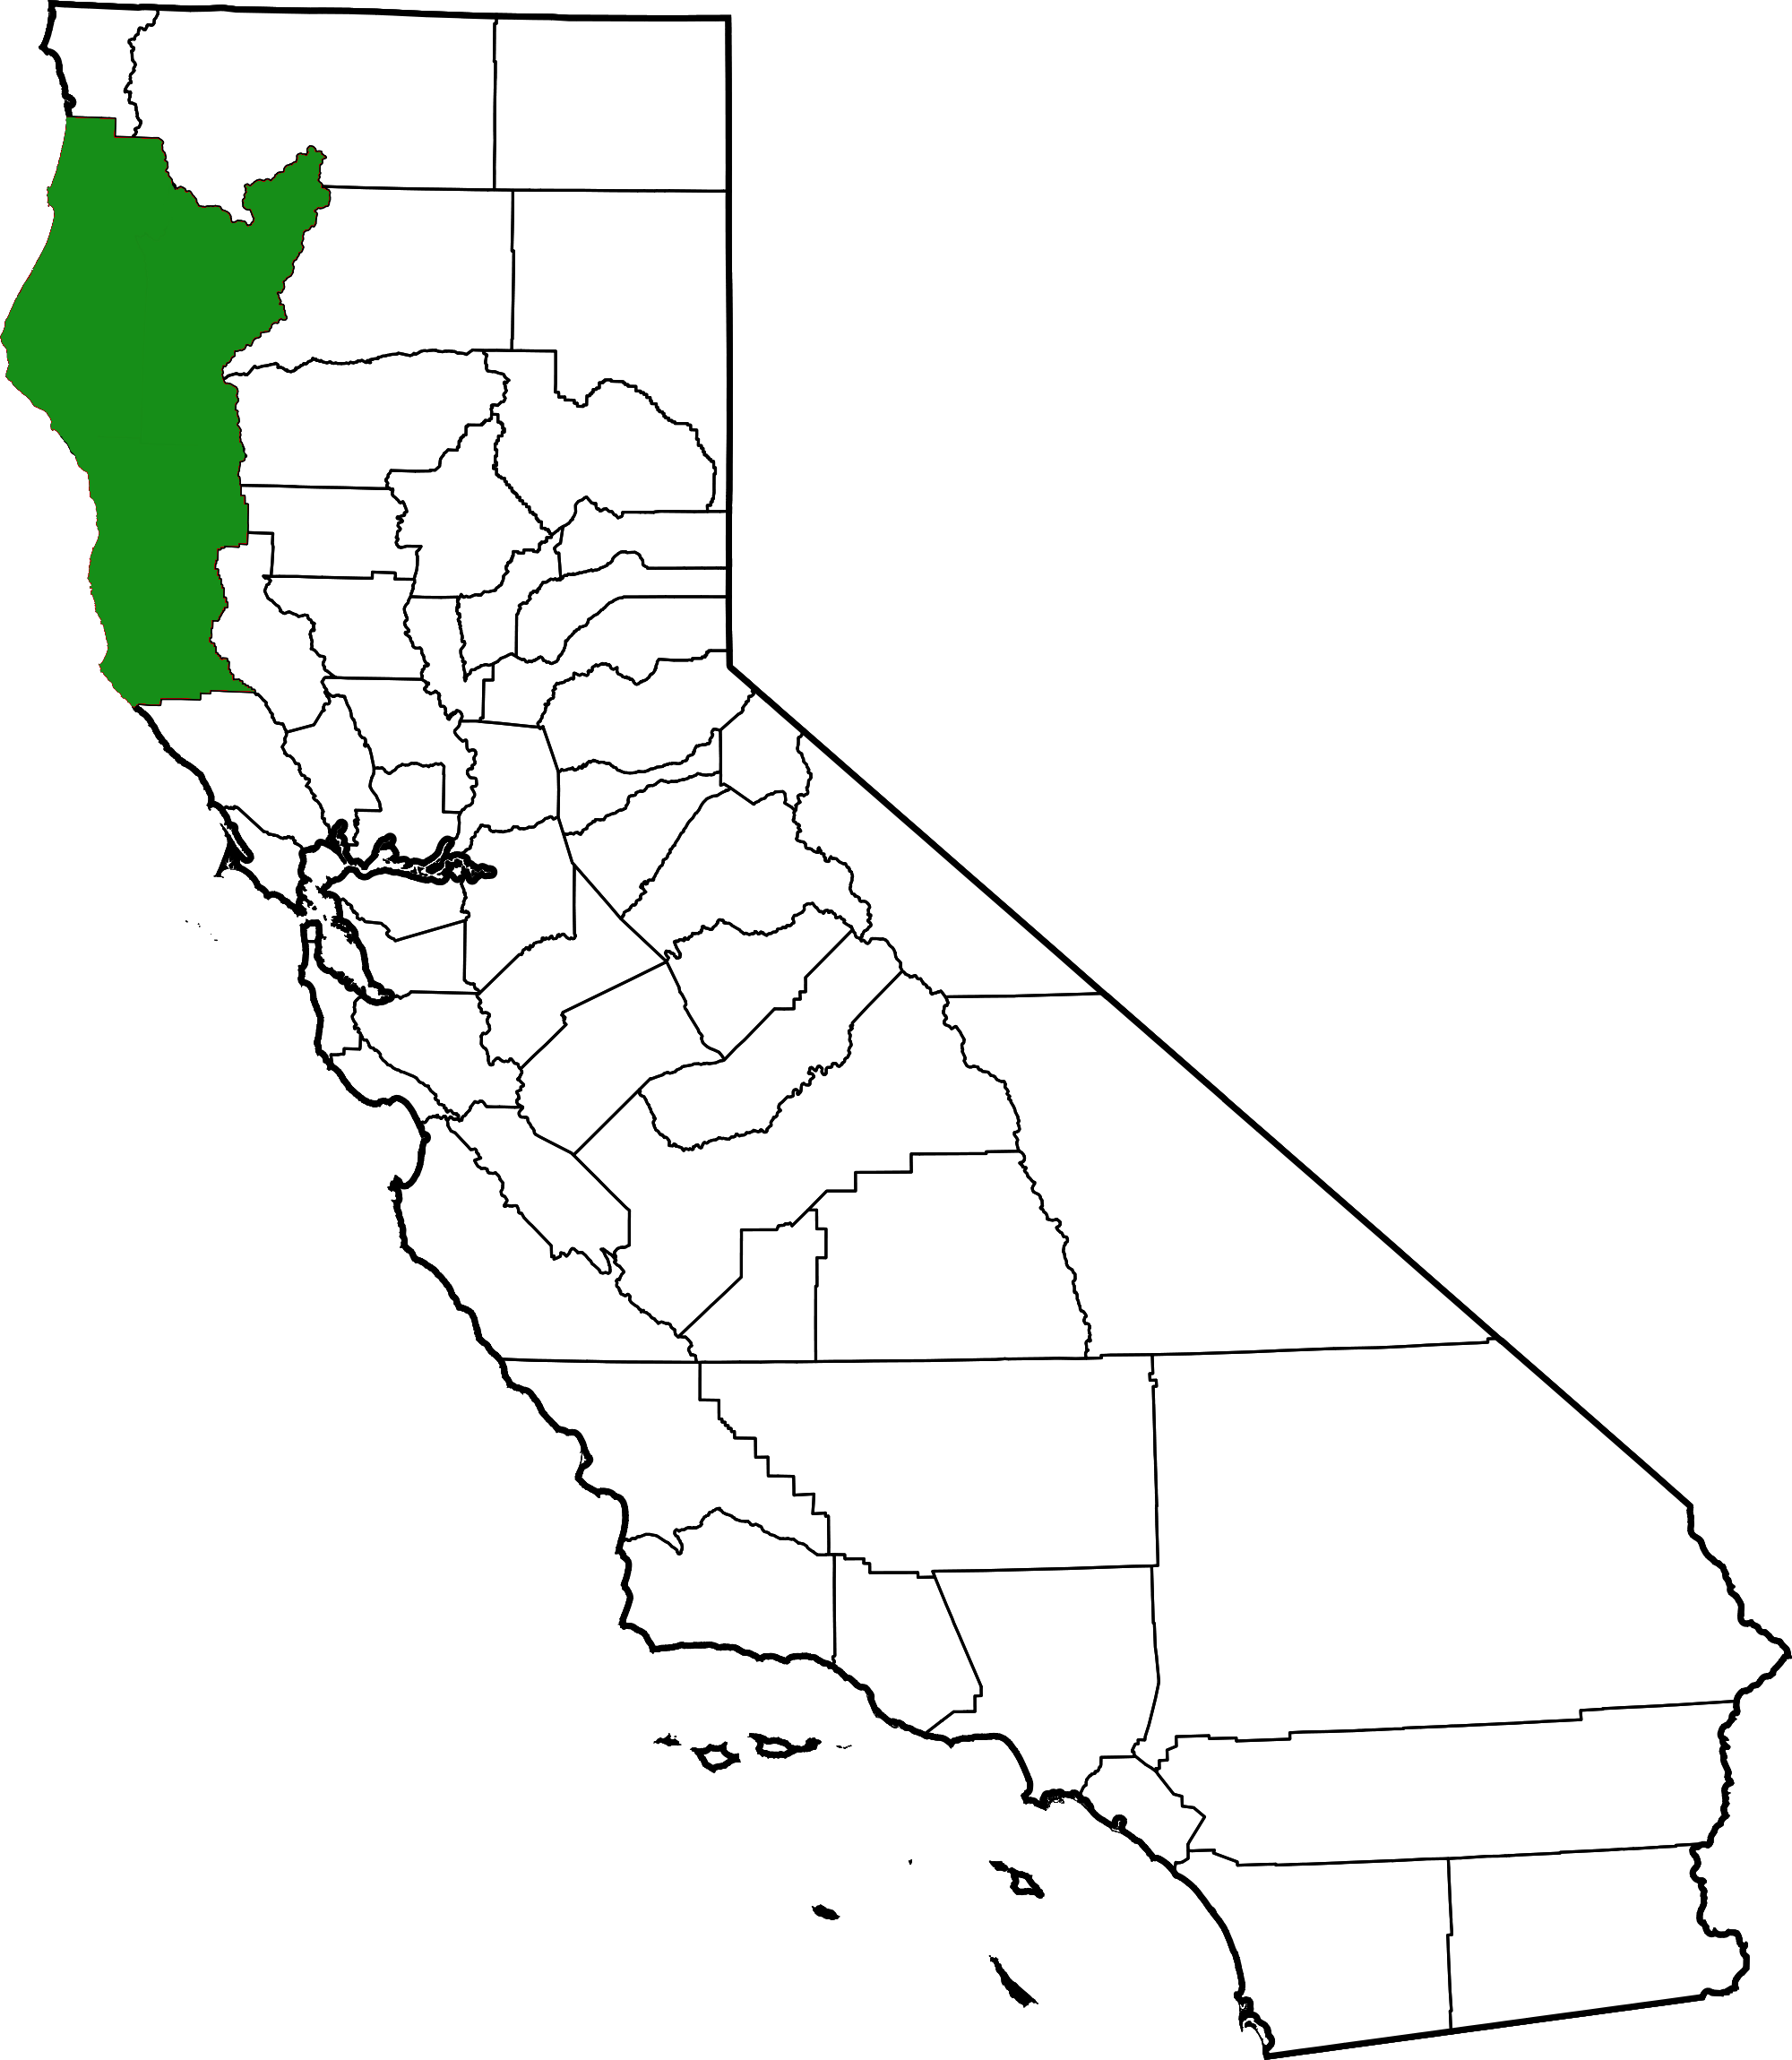
\includegraphics[width=\textwidth]{images/emerald-triangle.png}\\
    {\tiny O'Dea at Wikimedia Commons, CC BY-SA 4.0}
\end{figure}
\end{minipage}

\end{frame}


%------------------------------------------%
% The Emerald Cup
%------------------------------------------%

\begin{frame}{The Emerald Cup}

\vspace*{0.25\baselineskip}
\begin{center}
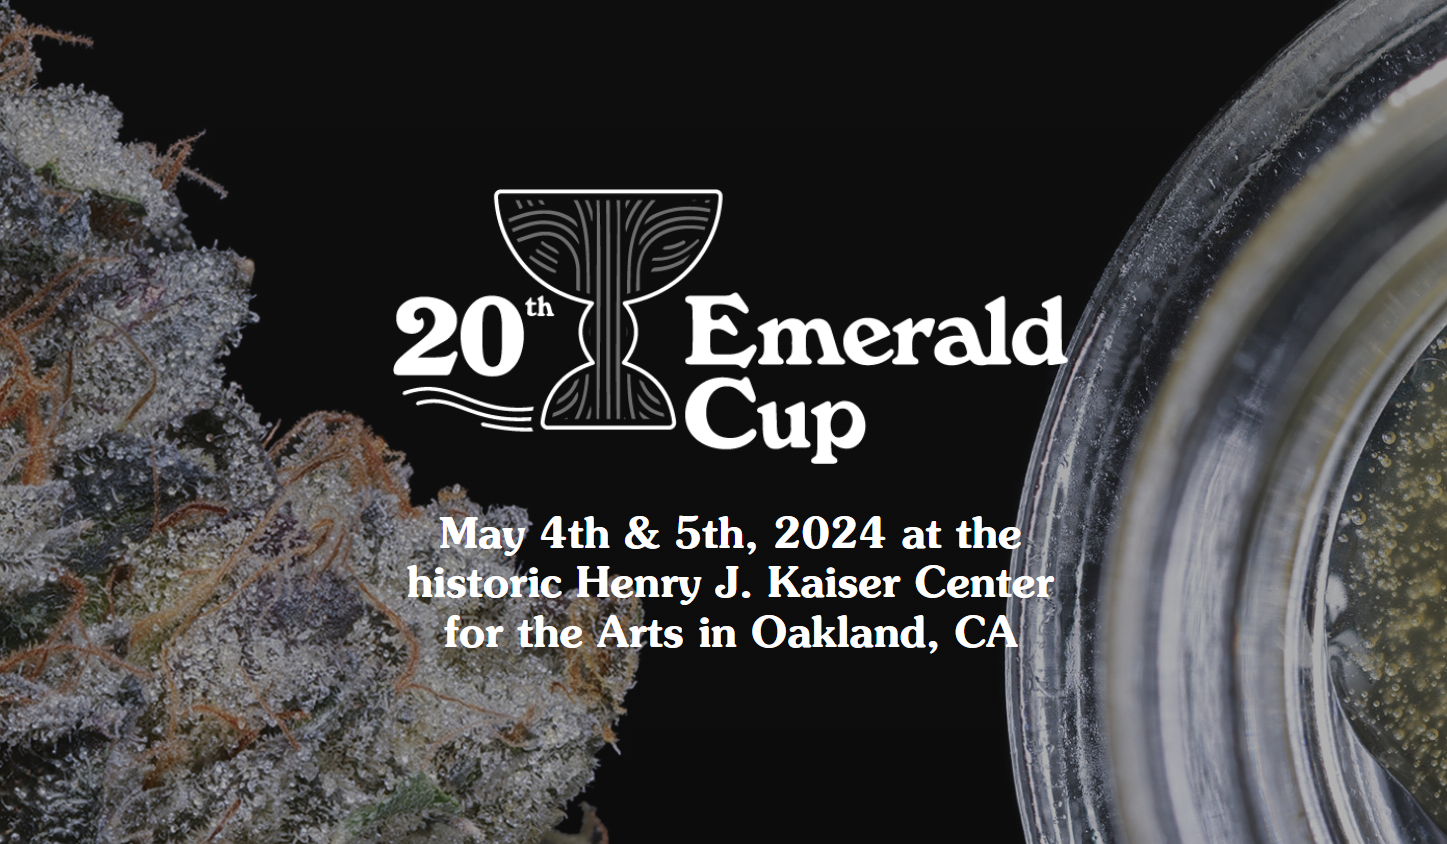
\includegraphics[width=0.9\textwidth]{images/emerald-cup-2024.png}
\end{center}
\vspace*{0.25\baselineskip}


\textcolor{OliveGreen}{\bfseries Emerald Cup Data}
\vspace*{0.125\baselineskip}
{\small
\begin{itemize}
\item 2022 winners: https://theemeraldcup.com/2022-award-winners
\item 2023 winners: https://theemeraldcup.com/2023-award-winners
\item SC Labs results: https://client.sclabs.com/verify/
\end{itemize}
}

\end{frame}


% News source: https://www.forbes.com/sites/lindseybartlett/2023/05/16/the-emerald-cup-celebrates-its-2023-cannabis-award-winners-with-heart/?sh=57fcfbef3abc


%------------------------------------------%
% Highest terpene content
%------------------------------------------%

\begin{frame}

\textbf{2022 Highest Terpene Content}\newline Woodwide Farms – Mendo Crumble\\
{\itshape 4.2412\% total terpenes}

\begin{figure}[h]
\centering
\includegraphics[width=0.45\textwidth]{images/mendo-crumble.png}
\end{figure}

\textbf{2023 Highest Terpene Content}\newline Sanctuary Farms – Blunicorn\\
{\itshape 4.9194\% total terpenes} \textcolor{OliveGreen}{(+15.99\%)}

\begin{figure}[h]
\centering
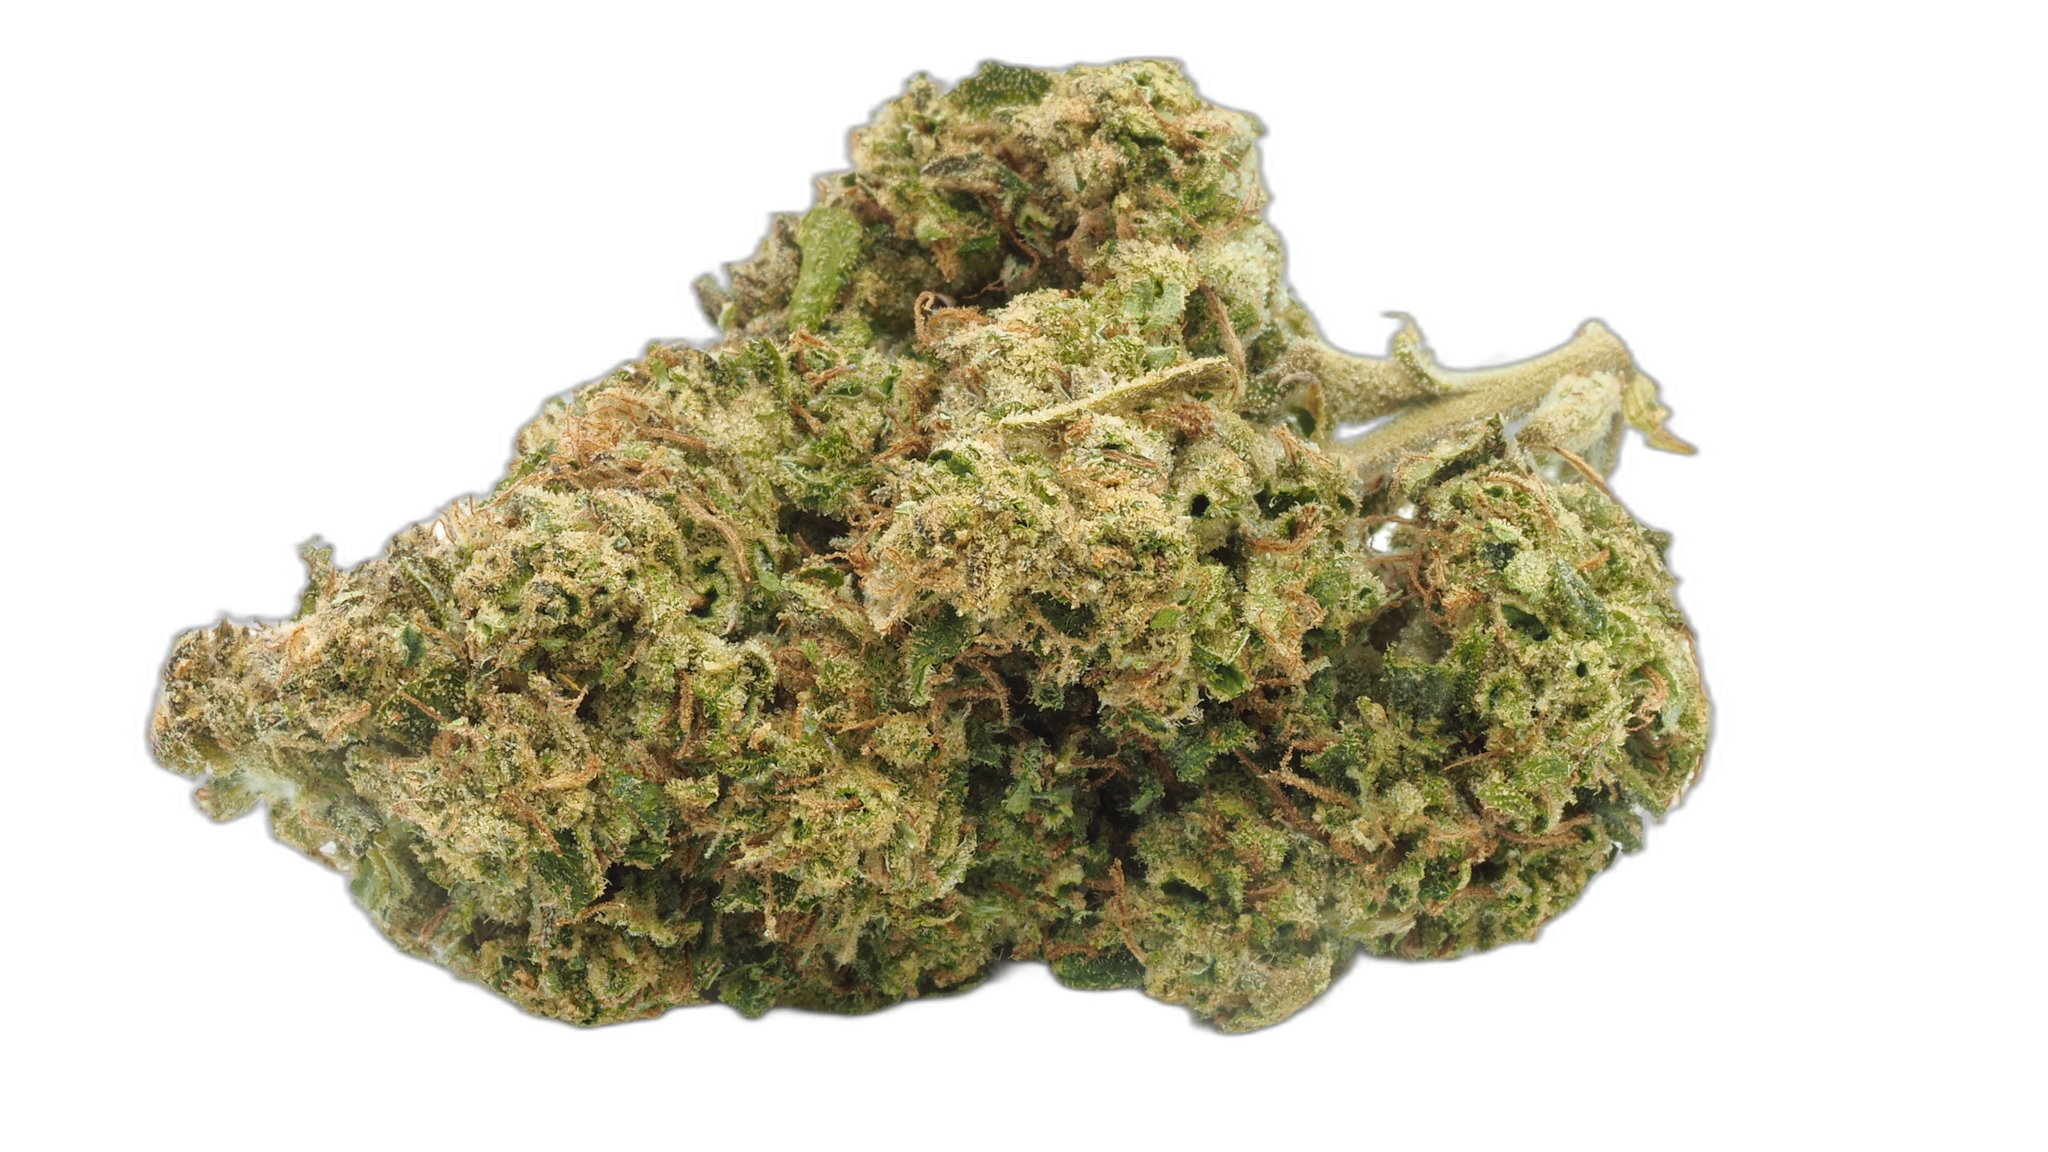
\includegraphics[width=0.45\textwidth]{images/blunicorn.png}
\end{figure}

\end{frame}


%------------------------------------------%
% Most Unique Terpene Profile
%------------------------------------------%

\begin{frame}{Most Unique Terpene Profile}

\begin{minipage}{0.45\textwidth}
\footnotesize
\includegraphics[width=0.8\textwidth]{images/waiting-game.png}\\
\textbf{2022 Predicted winner:} Waiting Game - Glasshouse Farms\\
\textit{Terpene diversity: 3.63}
\end{minipage}
\hfill
\begin{minipage}{0.45\textwidth}
\footnotesize
\includegraphics[width=0.8\textwidth]{images/juice-z.png}\\
\textbf{2022 Official winner:} Atrium Cultivation – Juice Z\\
\textit{Terpene diversity: 3.19}
\end{minipage}

\vspace{10pt}

\begin{minipage}{0.45\textwidth}
\footnotesize
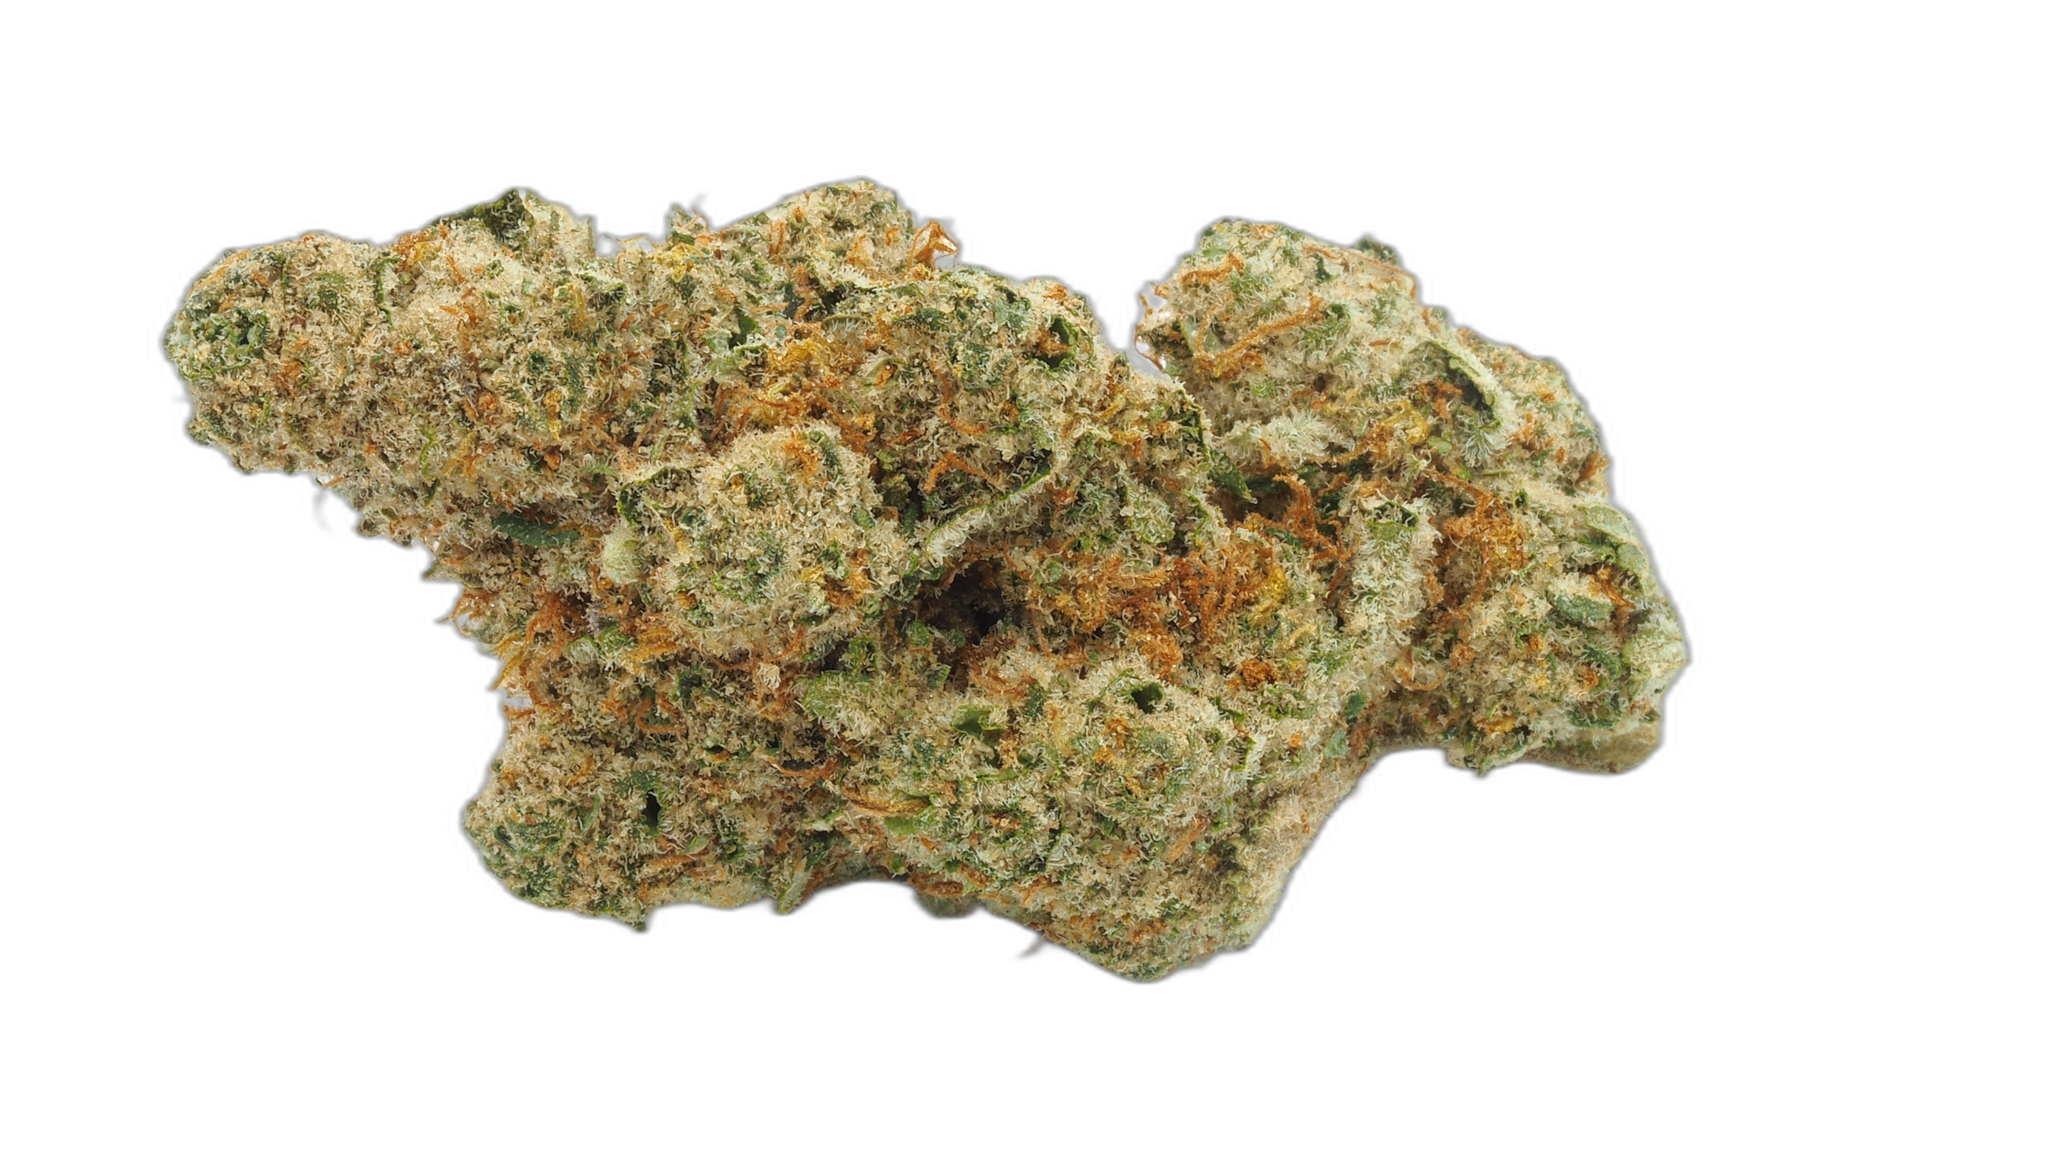
\includegraphics[width=0.8\textwidth]{images/strawberry-jam.png}\\
\textbf{2023 Predicted winner:} Fog City Farms - Strawberry Jam\\
\textit{Terpene diversity: 3.61}
\end{minipage}
\hfill
\begin{minipage}{0.45\textwidth}
\footnotesize
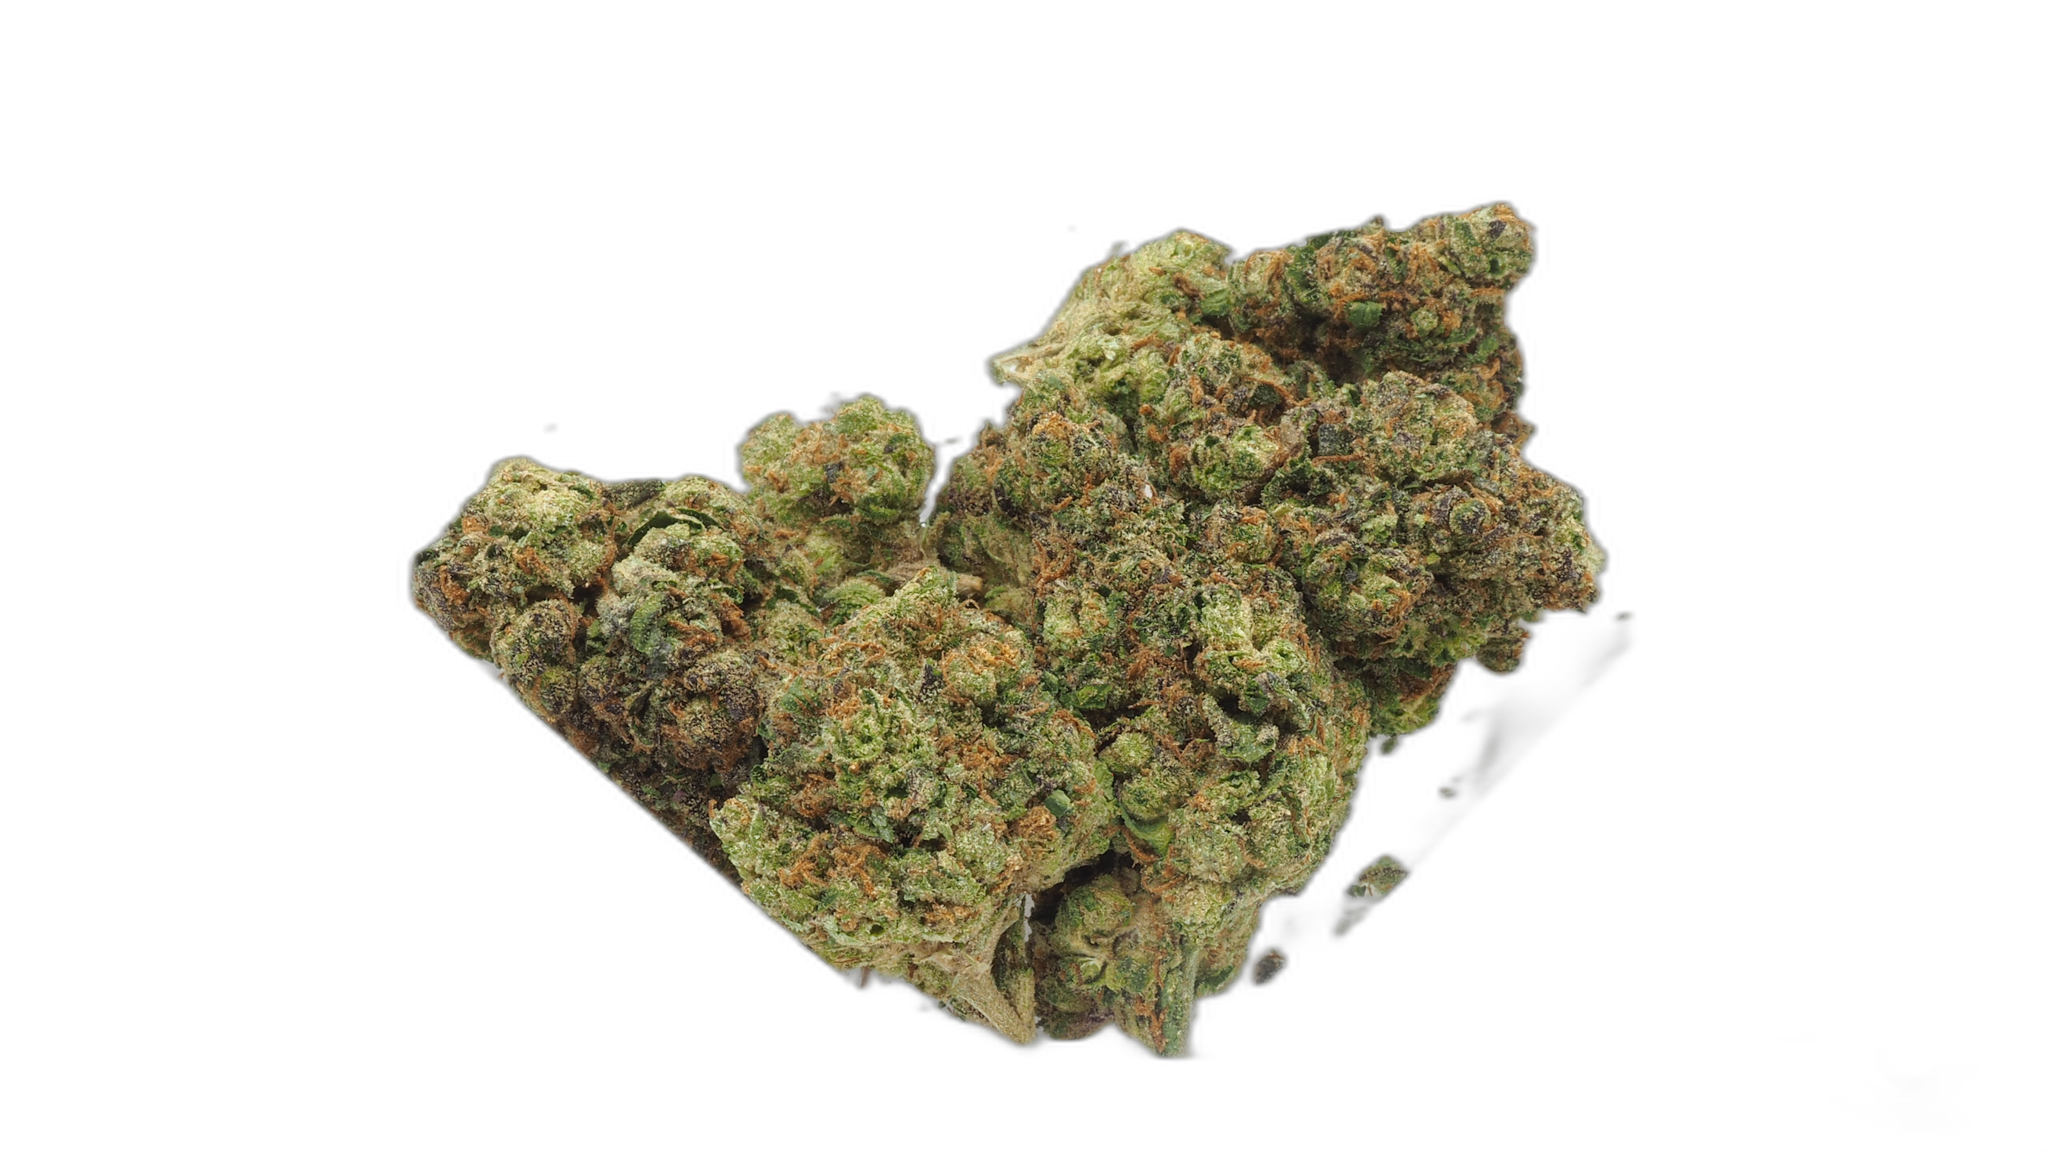
\includegraphics[width=0.8\textwidth]{images/lilac-mintz.png}\\
\textbf{2023 Official winner:} Healing Herb Farms – Lilac Mintz\\
\textit{Terpene diversity: 3.03}
\end{minipage}

\end{frame}


%------------------------------------------%
% Analysis
%------------------------------------------%

% Total Terpenes histogram
\begin{frame}{Total Terpenes}
  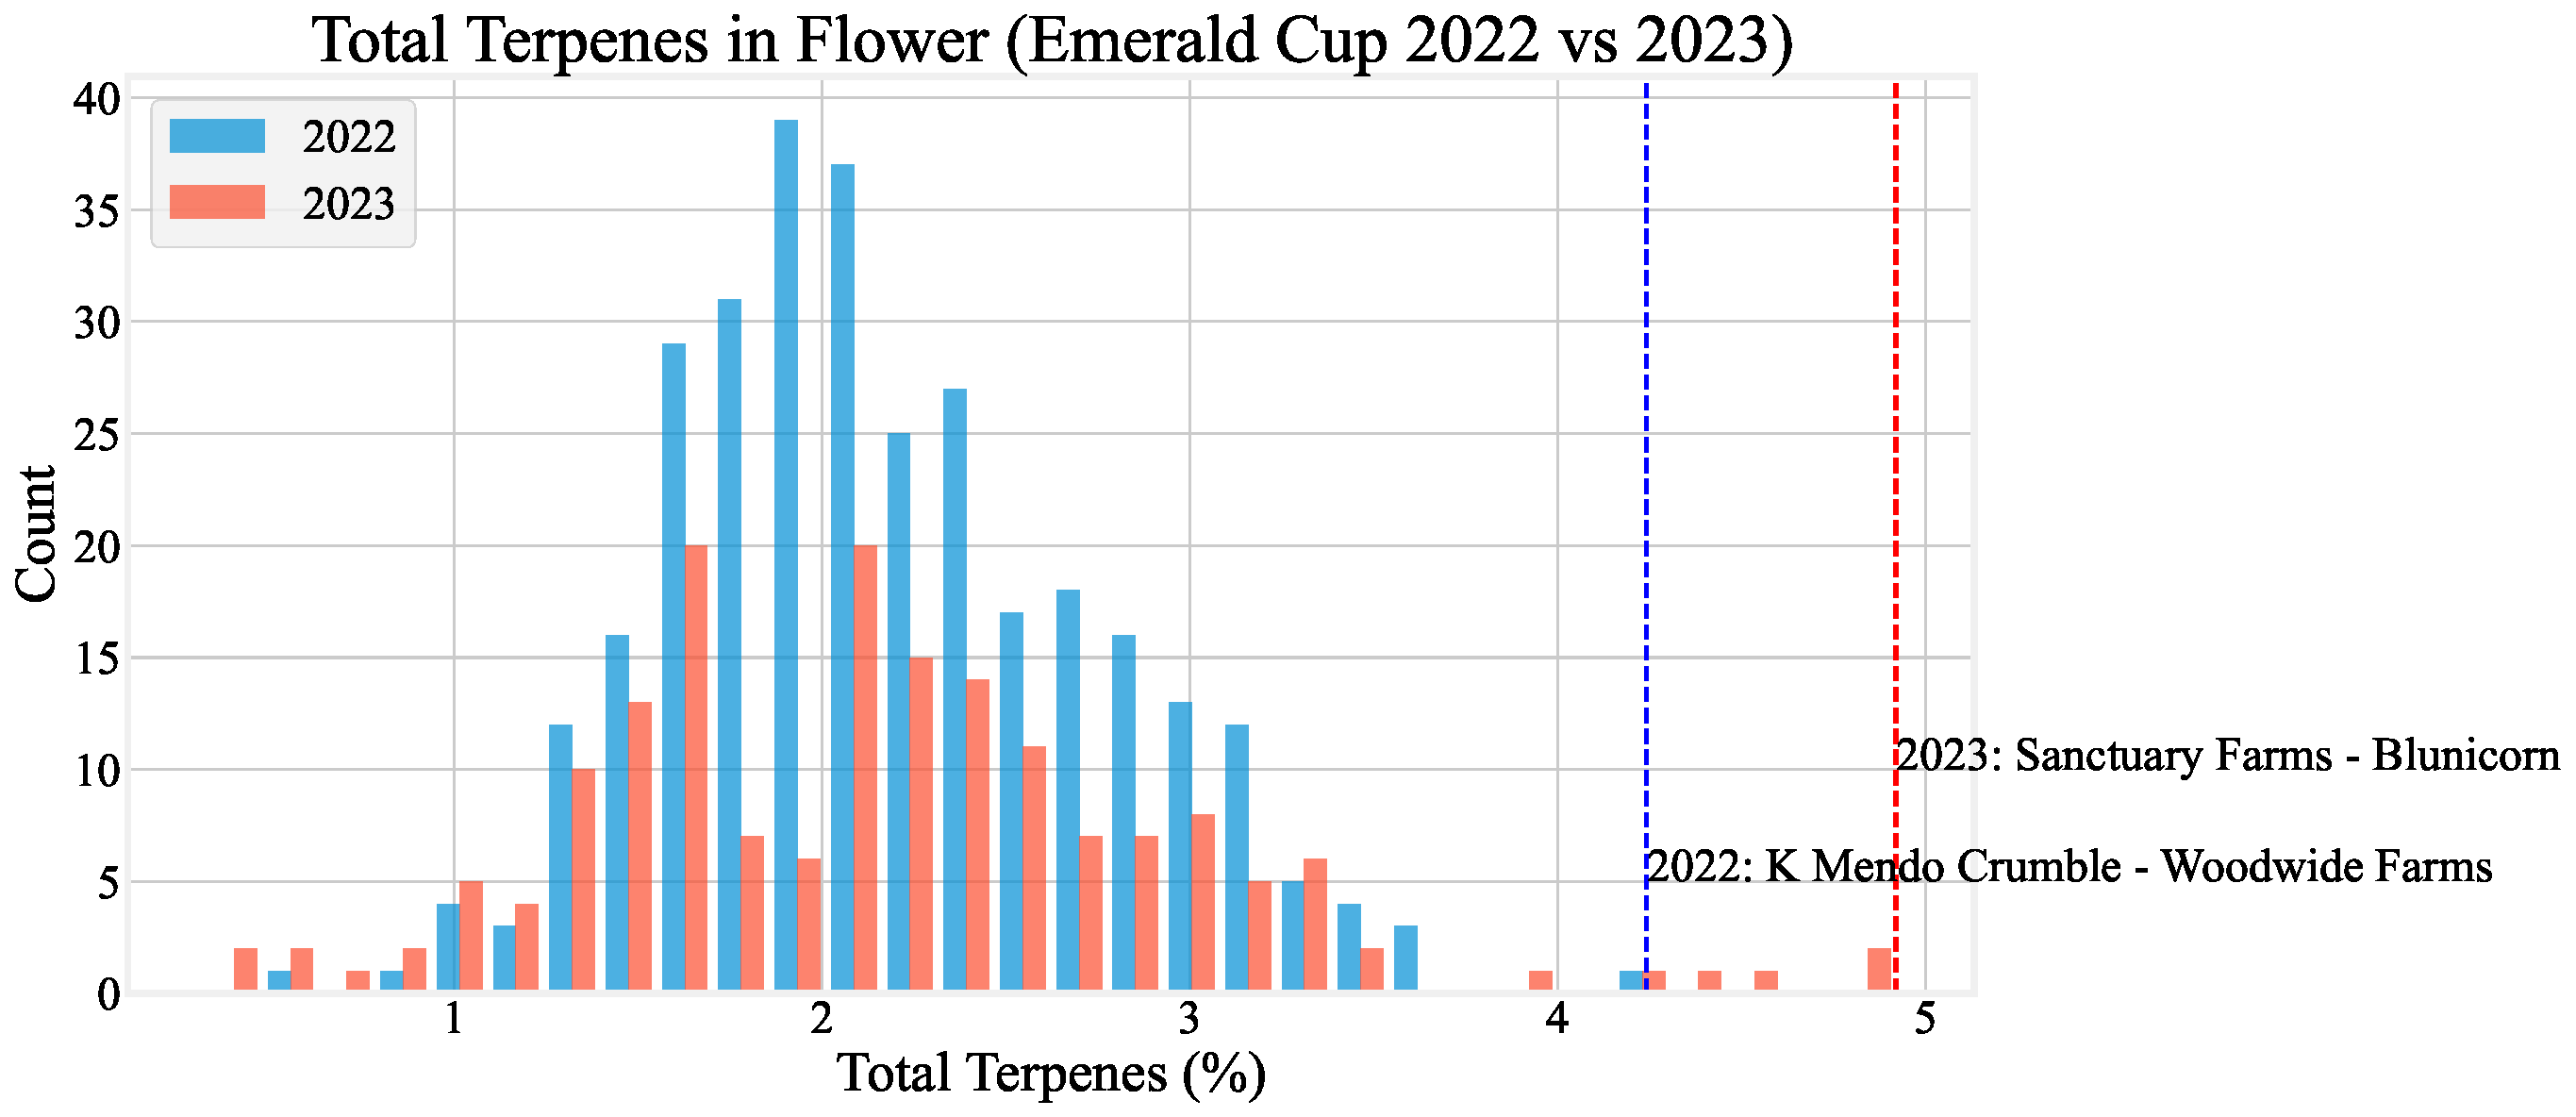
\includegraphics[width=\textwidth]{images/emerald-cup-total-terpenes-histogram.pdf}
\end{frame}

% Slide for Terpene diversity histogram
\begin{frame}{Terpene Diversity}
  \centering
  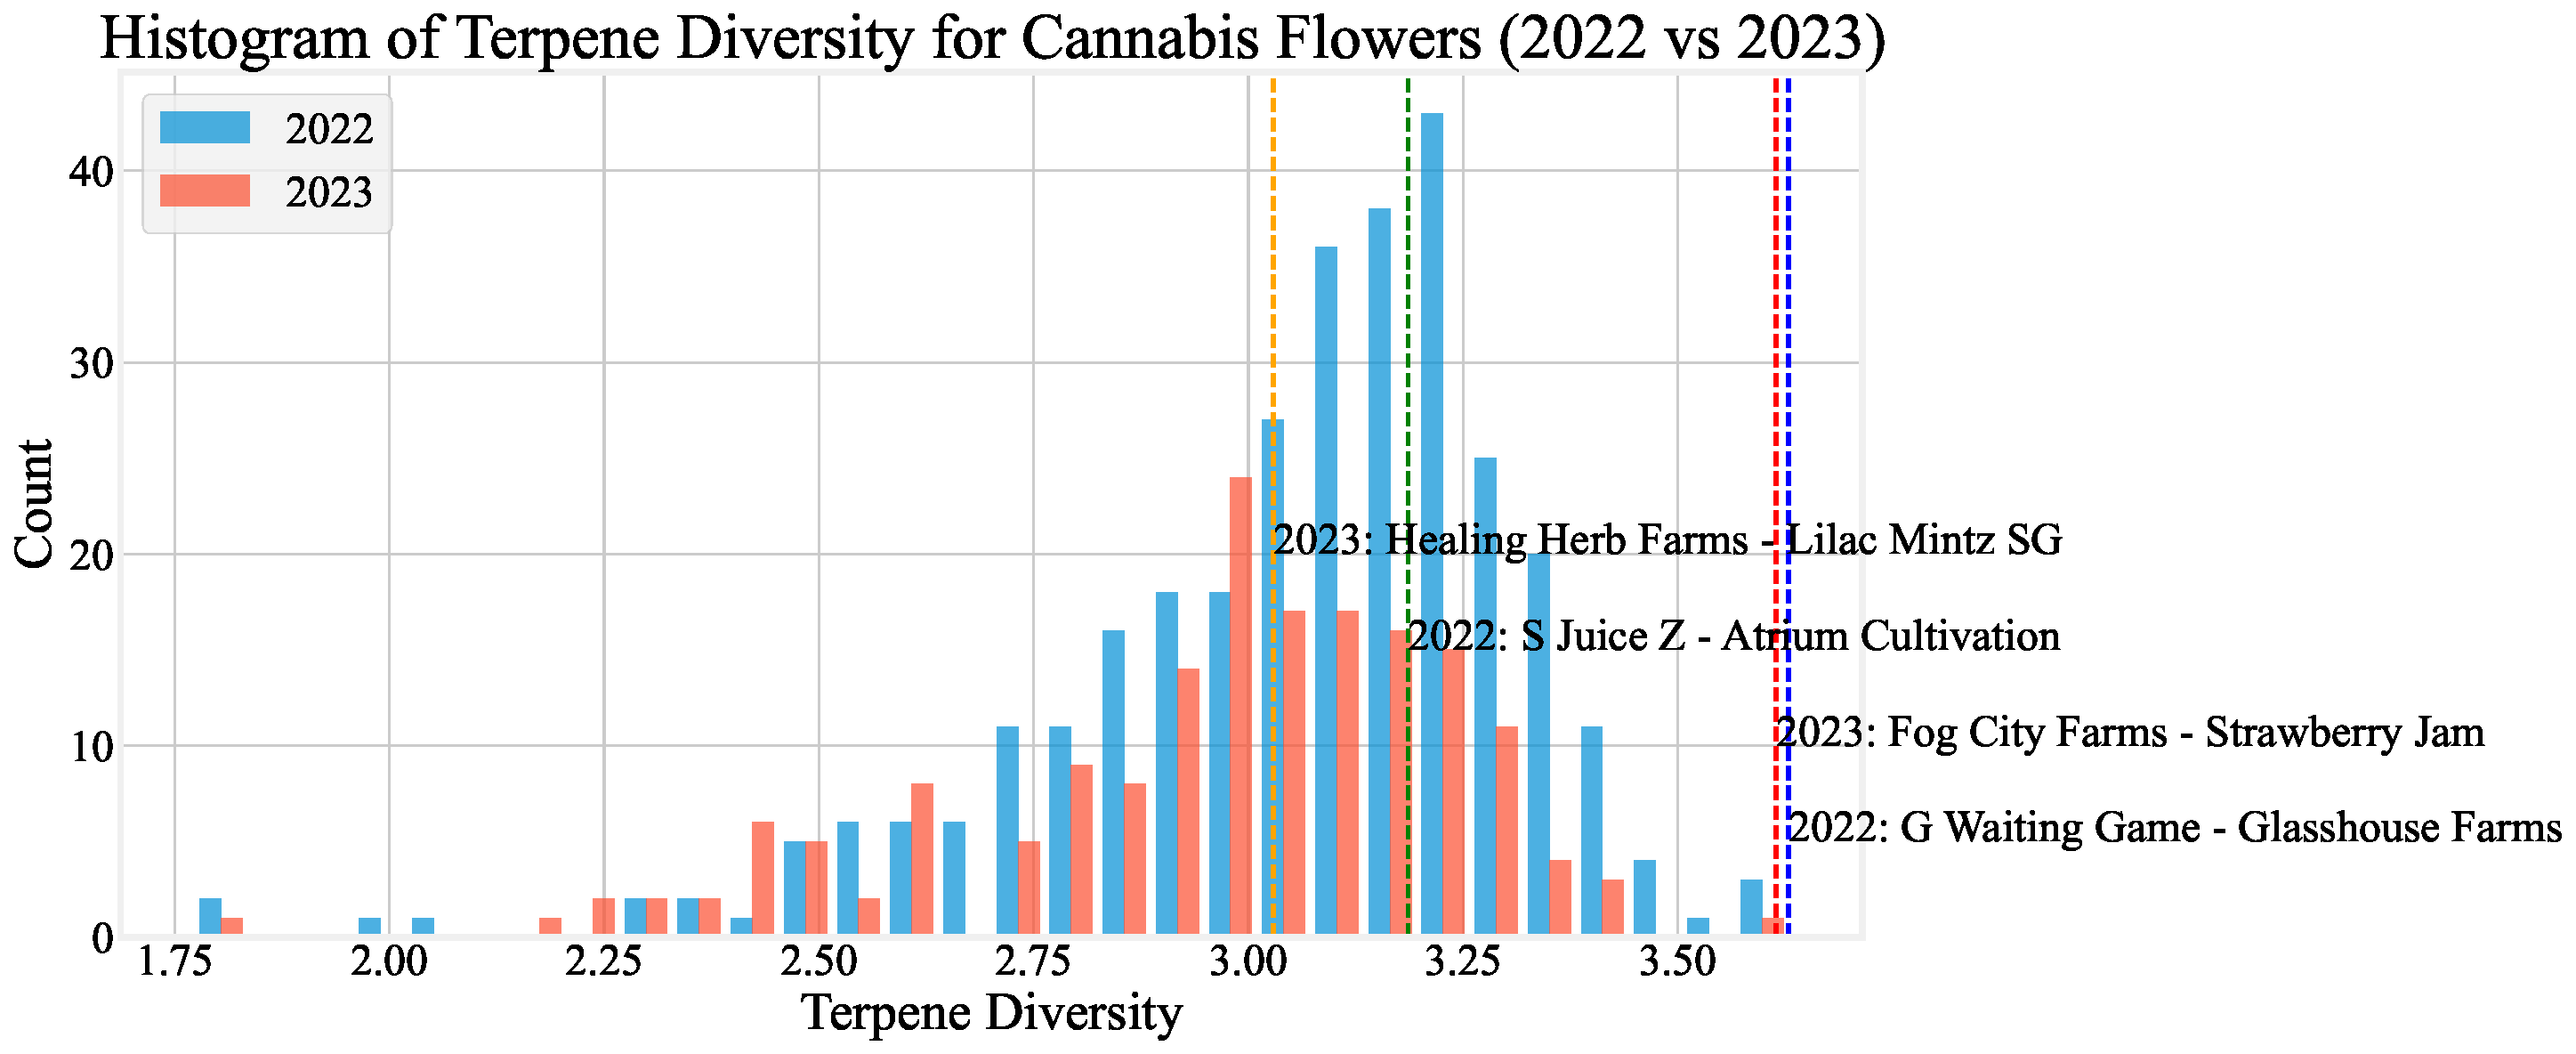
\includegraphics[width=\textwidth]{images/emerald-cup-terpene-diversity-histogram.pdf}
\end{frame}

% Terpene diversity barchart
\begin{frame}{Terpene Diversity}
  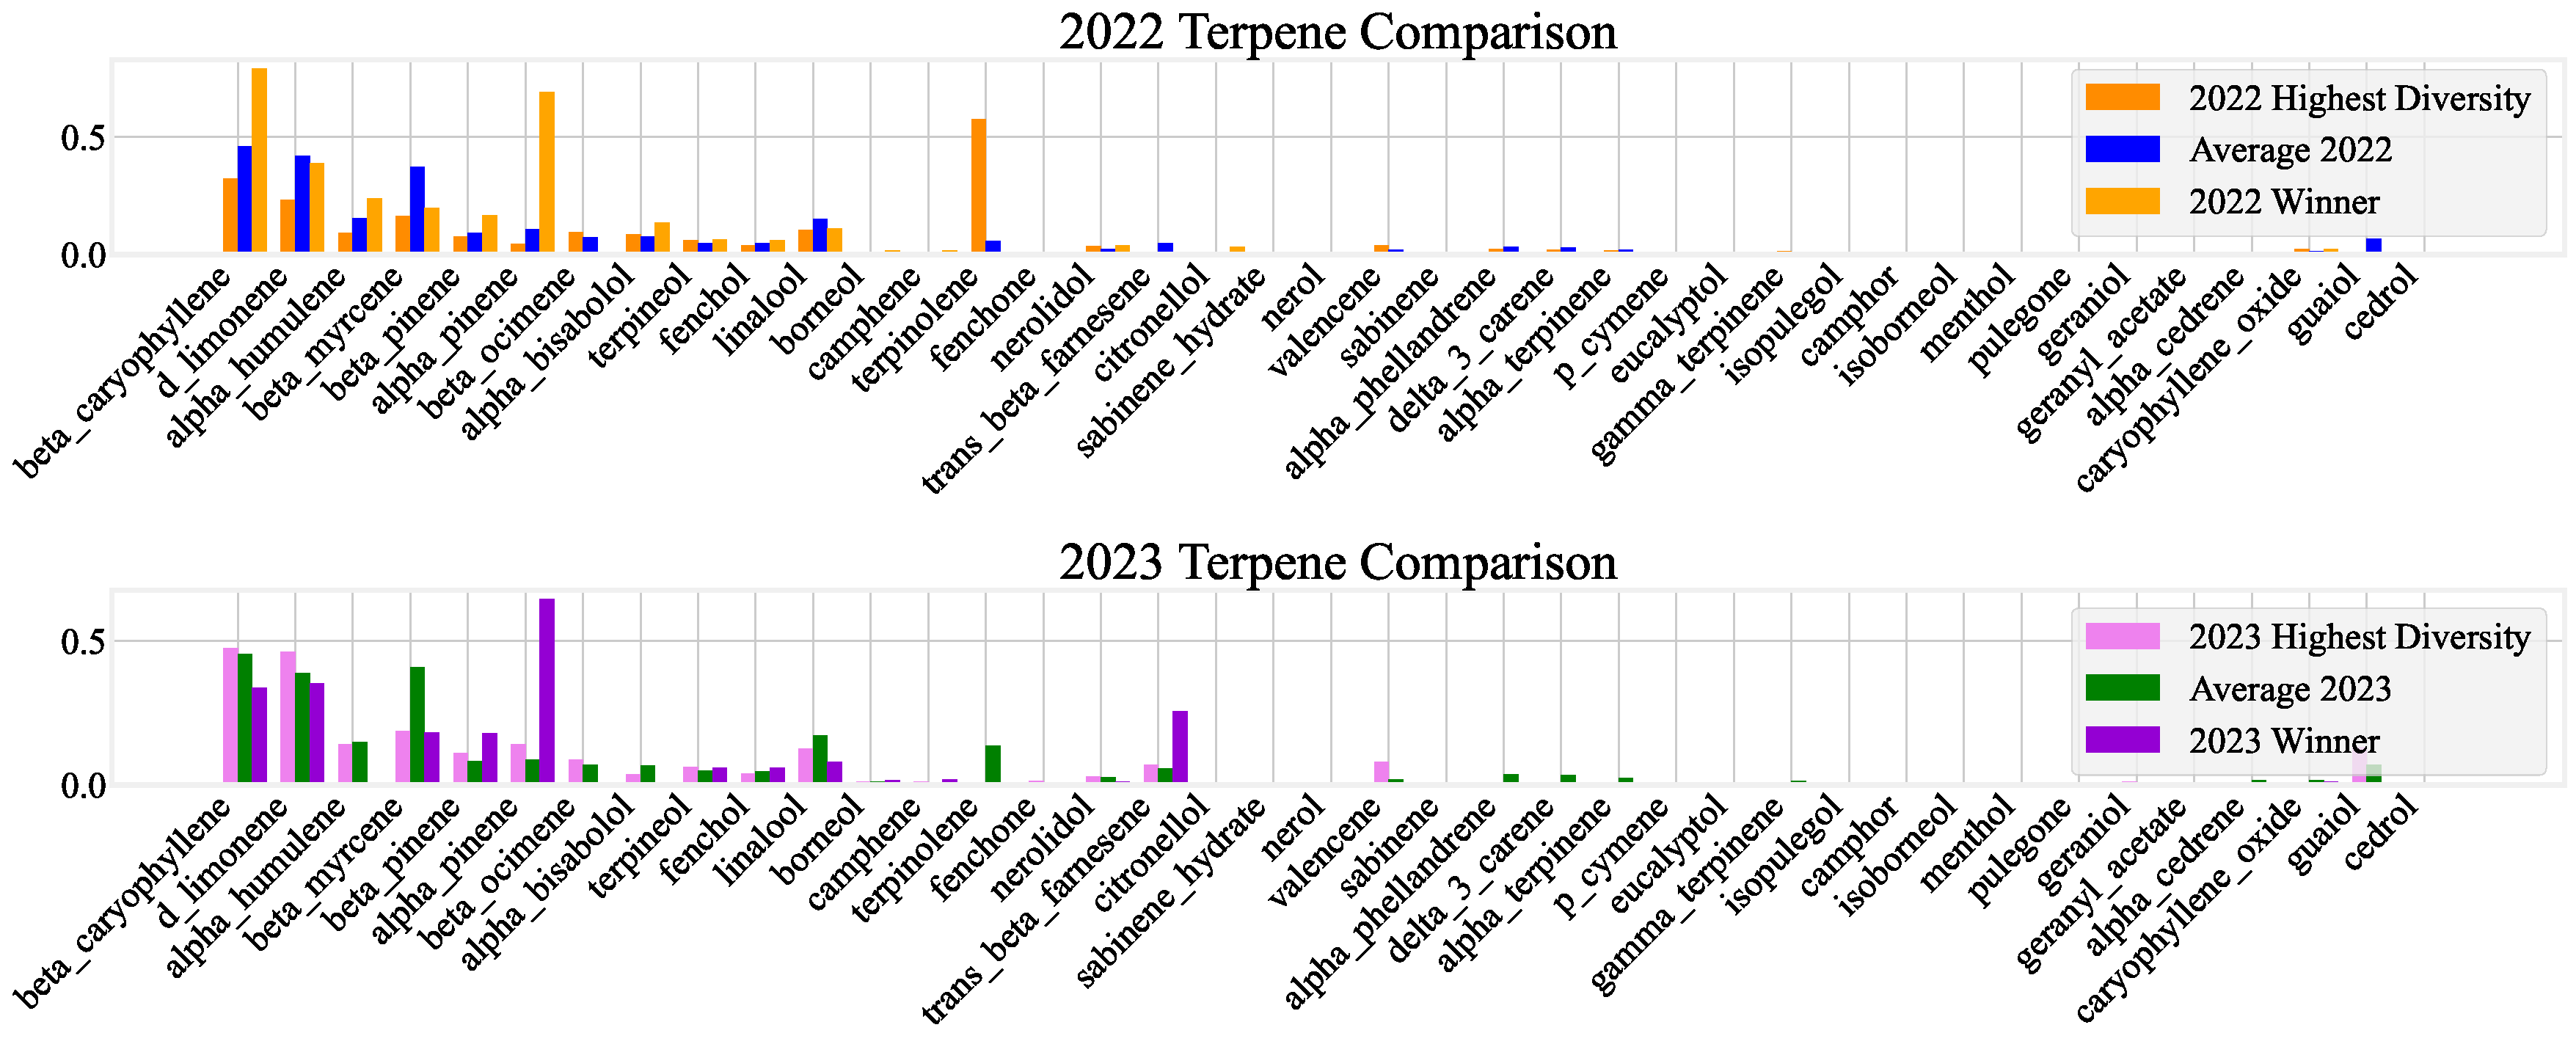
\includegraphics[width=\textwidth]{images/emerald-cup-terpene-diversity-winner.pdf}
\end{frame}

% Slide for Cannabinoid diversity histogram
\begin{frame}{Cannabinoid Diversity}
  \centering
  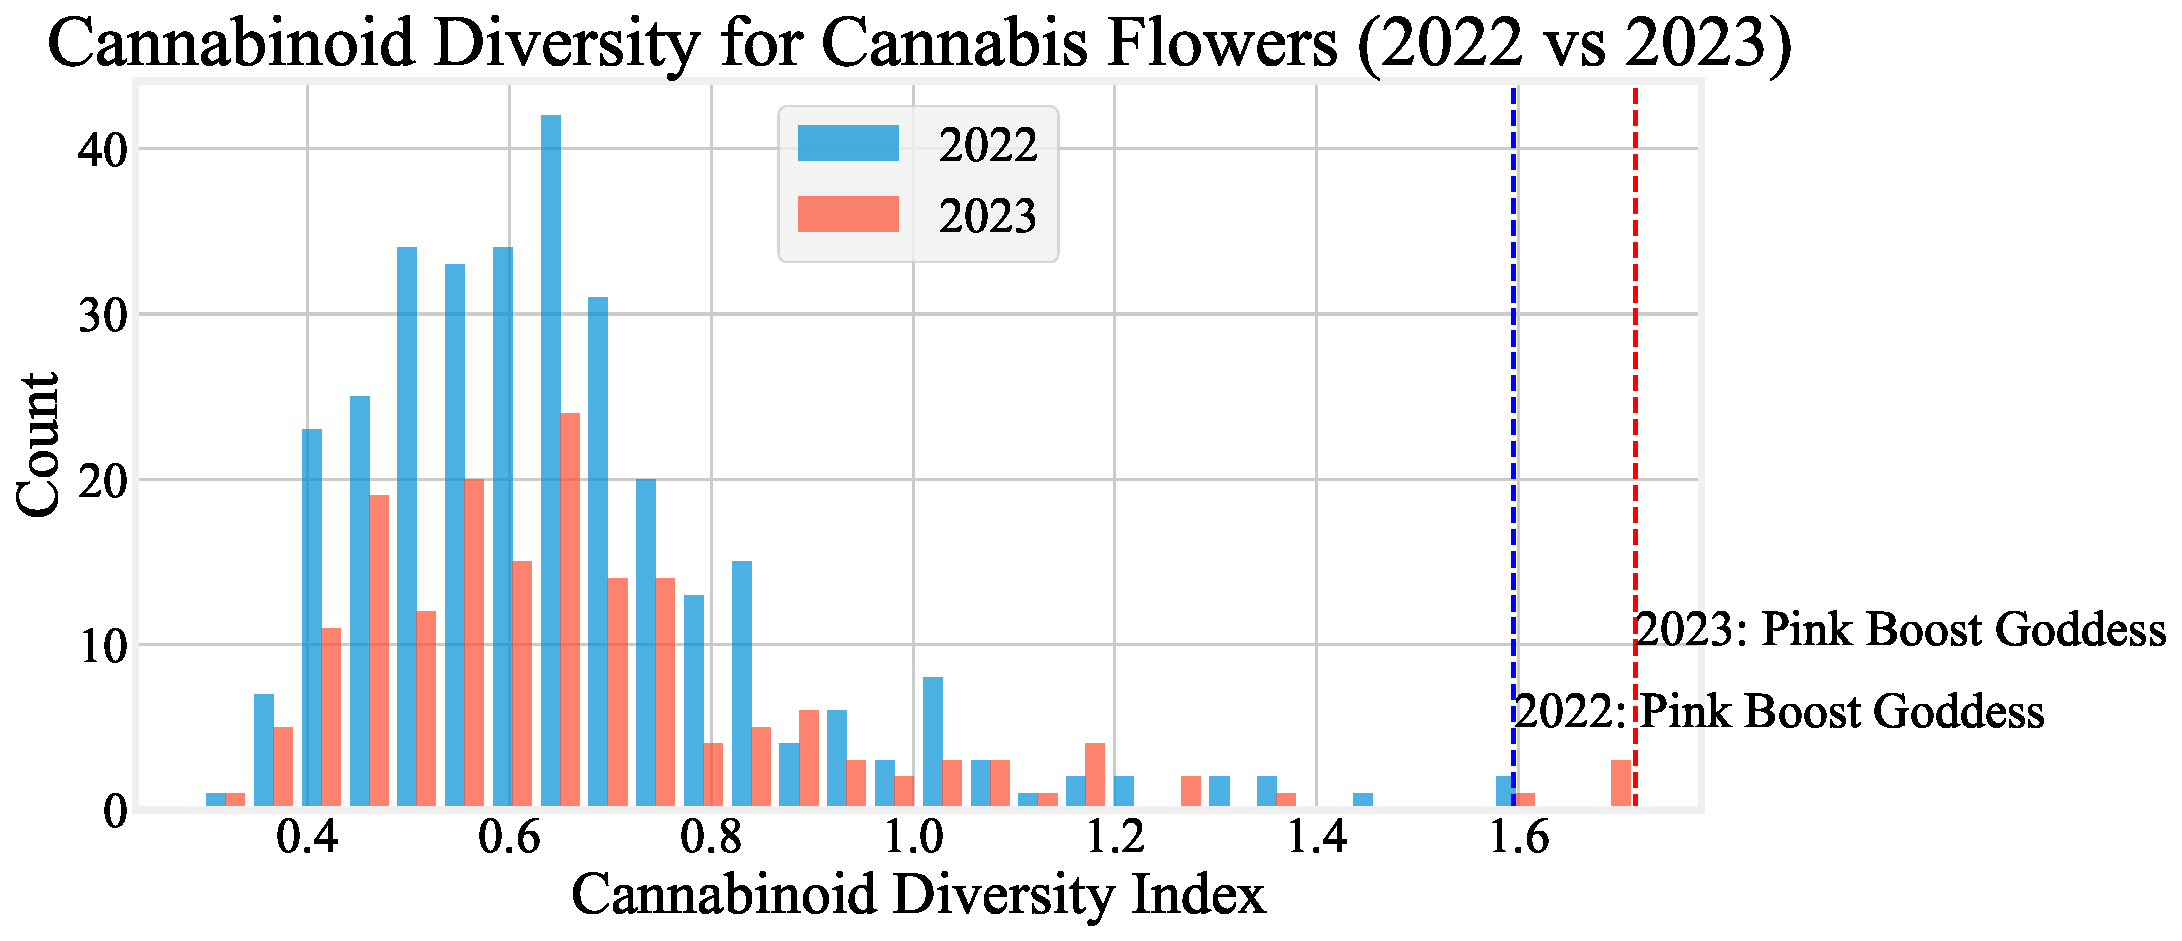
\includegraphics[width=\textwidth]{images/emerald-cup-cannabinoid-diversity-histogram.pdf}
\end{frame}

% Slide for Cannabinoid diversity winner
\begin{frame}{Cannabinoid Diversity}
  \centering
  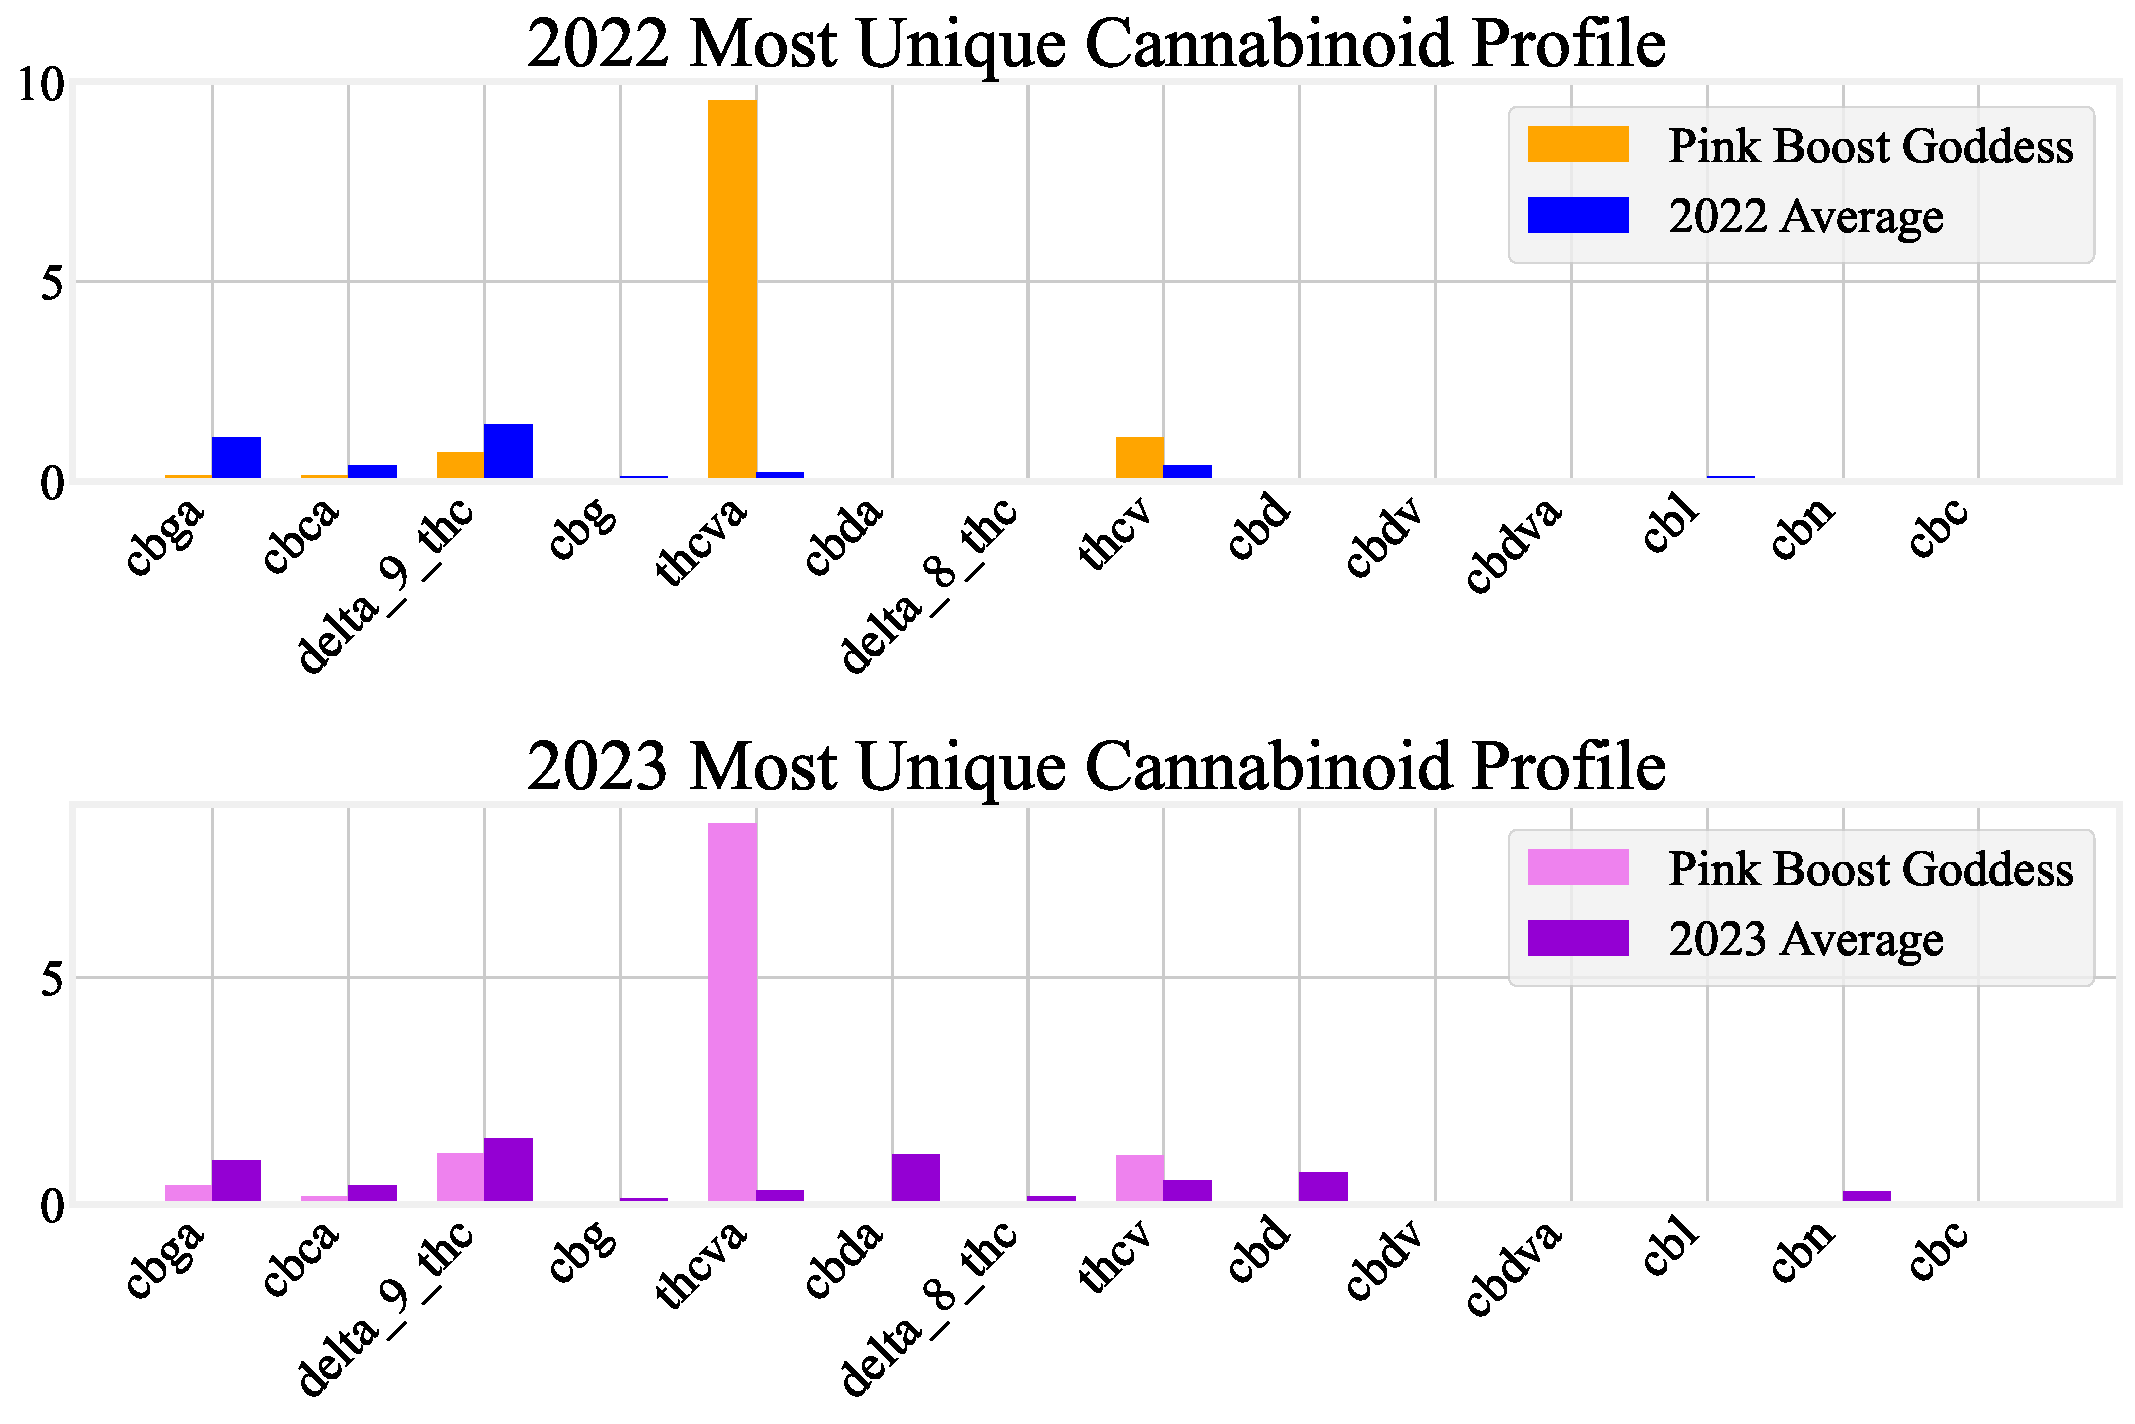
\includegraphics[width=\textwidth]{images/emerald-cup-cannabinoid-diversity-winner.pdf}
\end{frame}

% Slide for Purple scores
\begin{frame}{Purpleness}
  \centering
  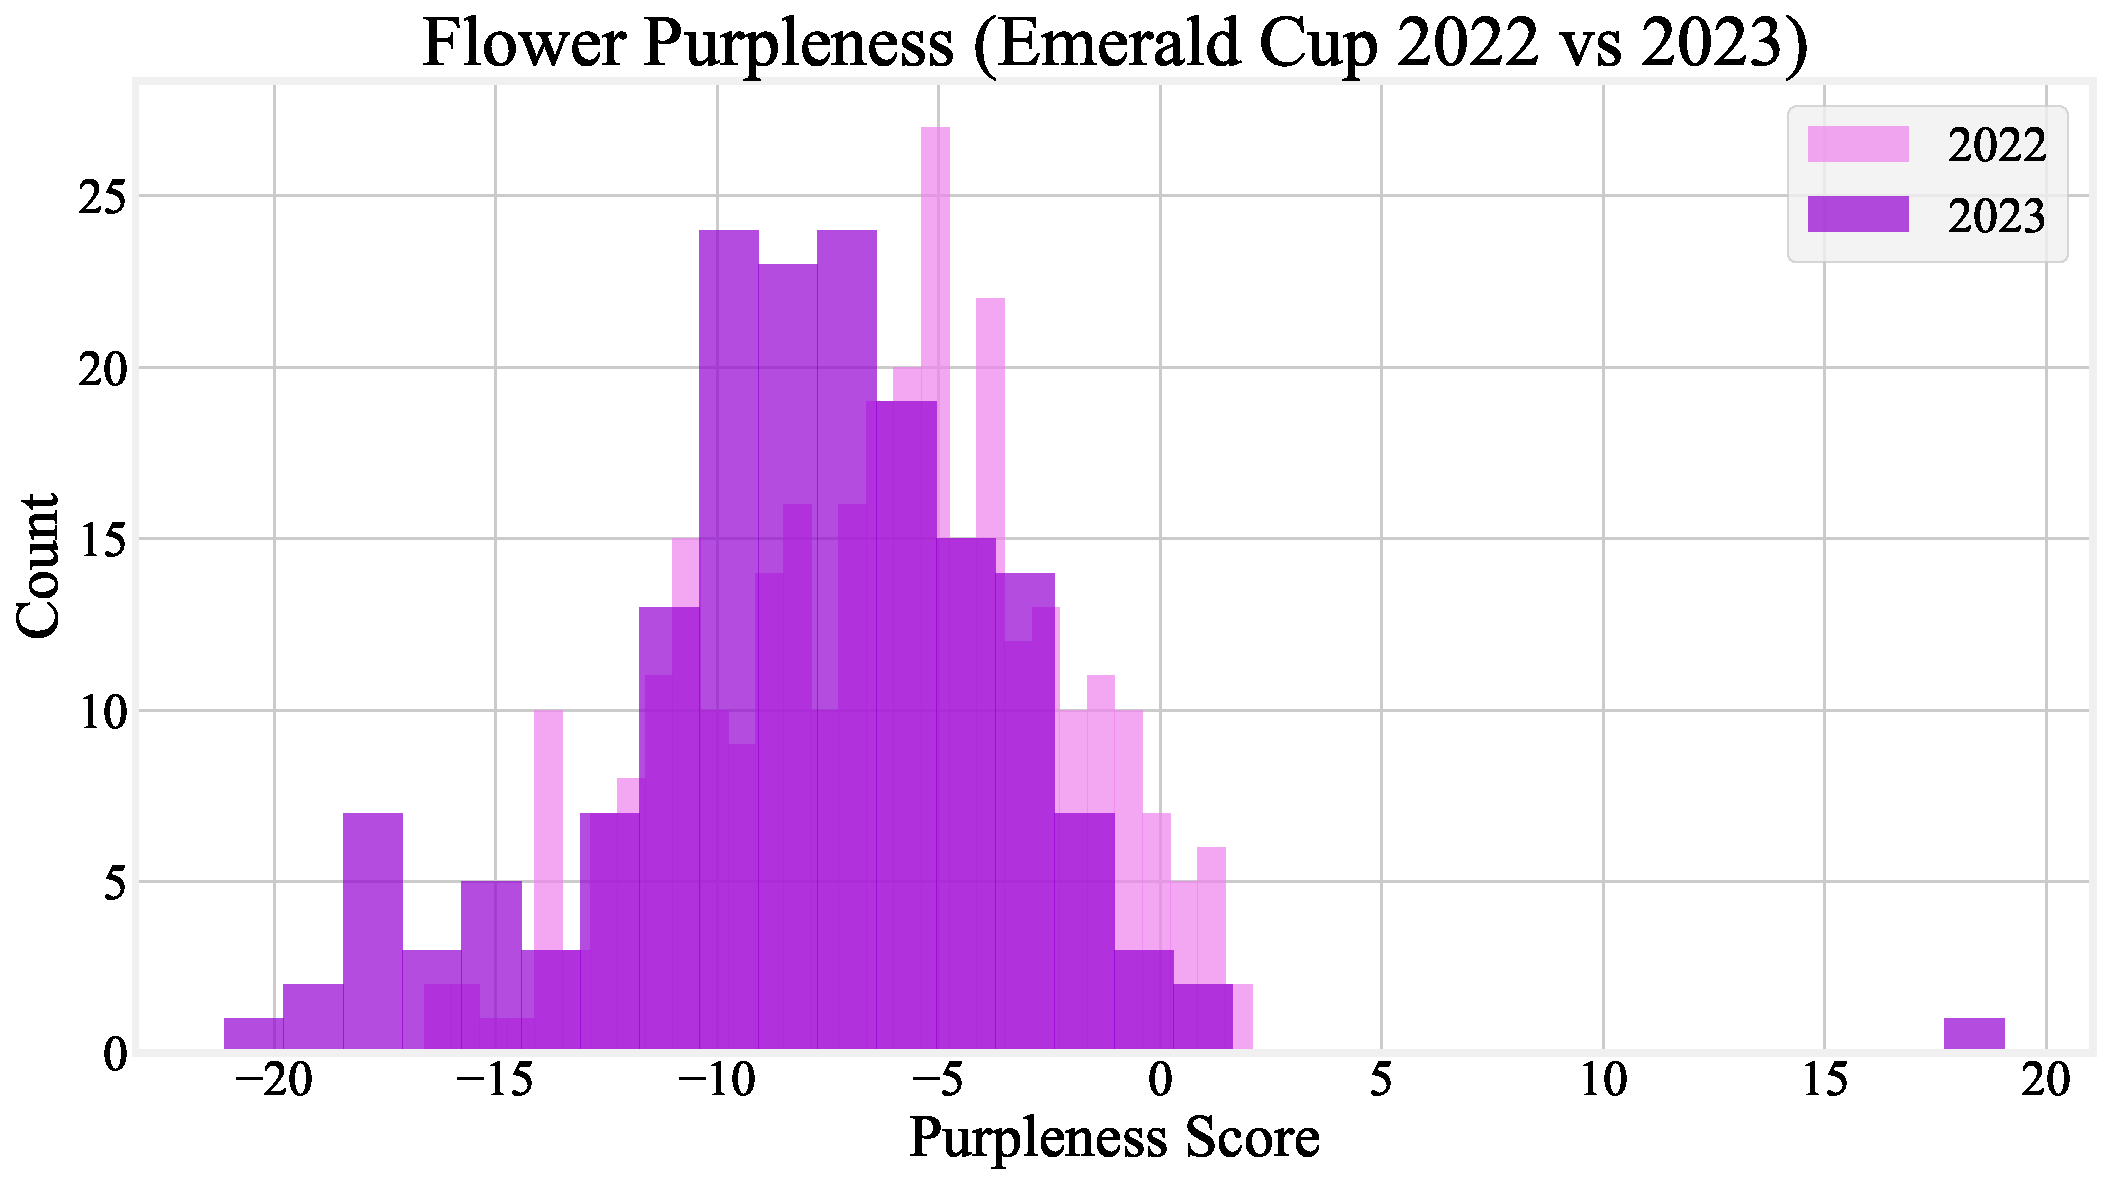
\includegraphics[width=\textwidth]{images/emerald-cup-purple-scores.pdf}
\end{frame}

% Slide for Colorfulness scores
\begin{frame}{Colorfulness Scores}
  \centering
  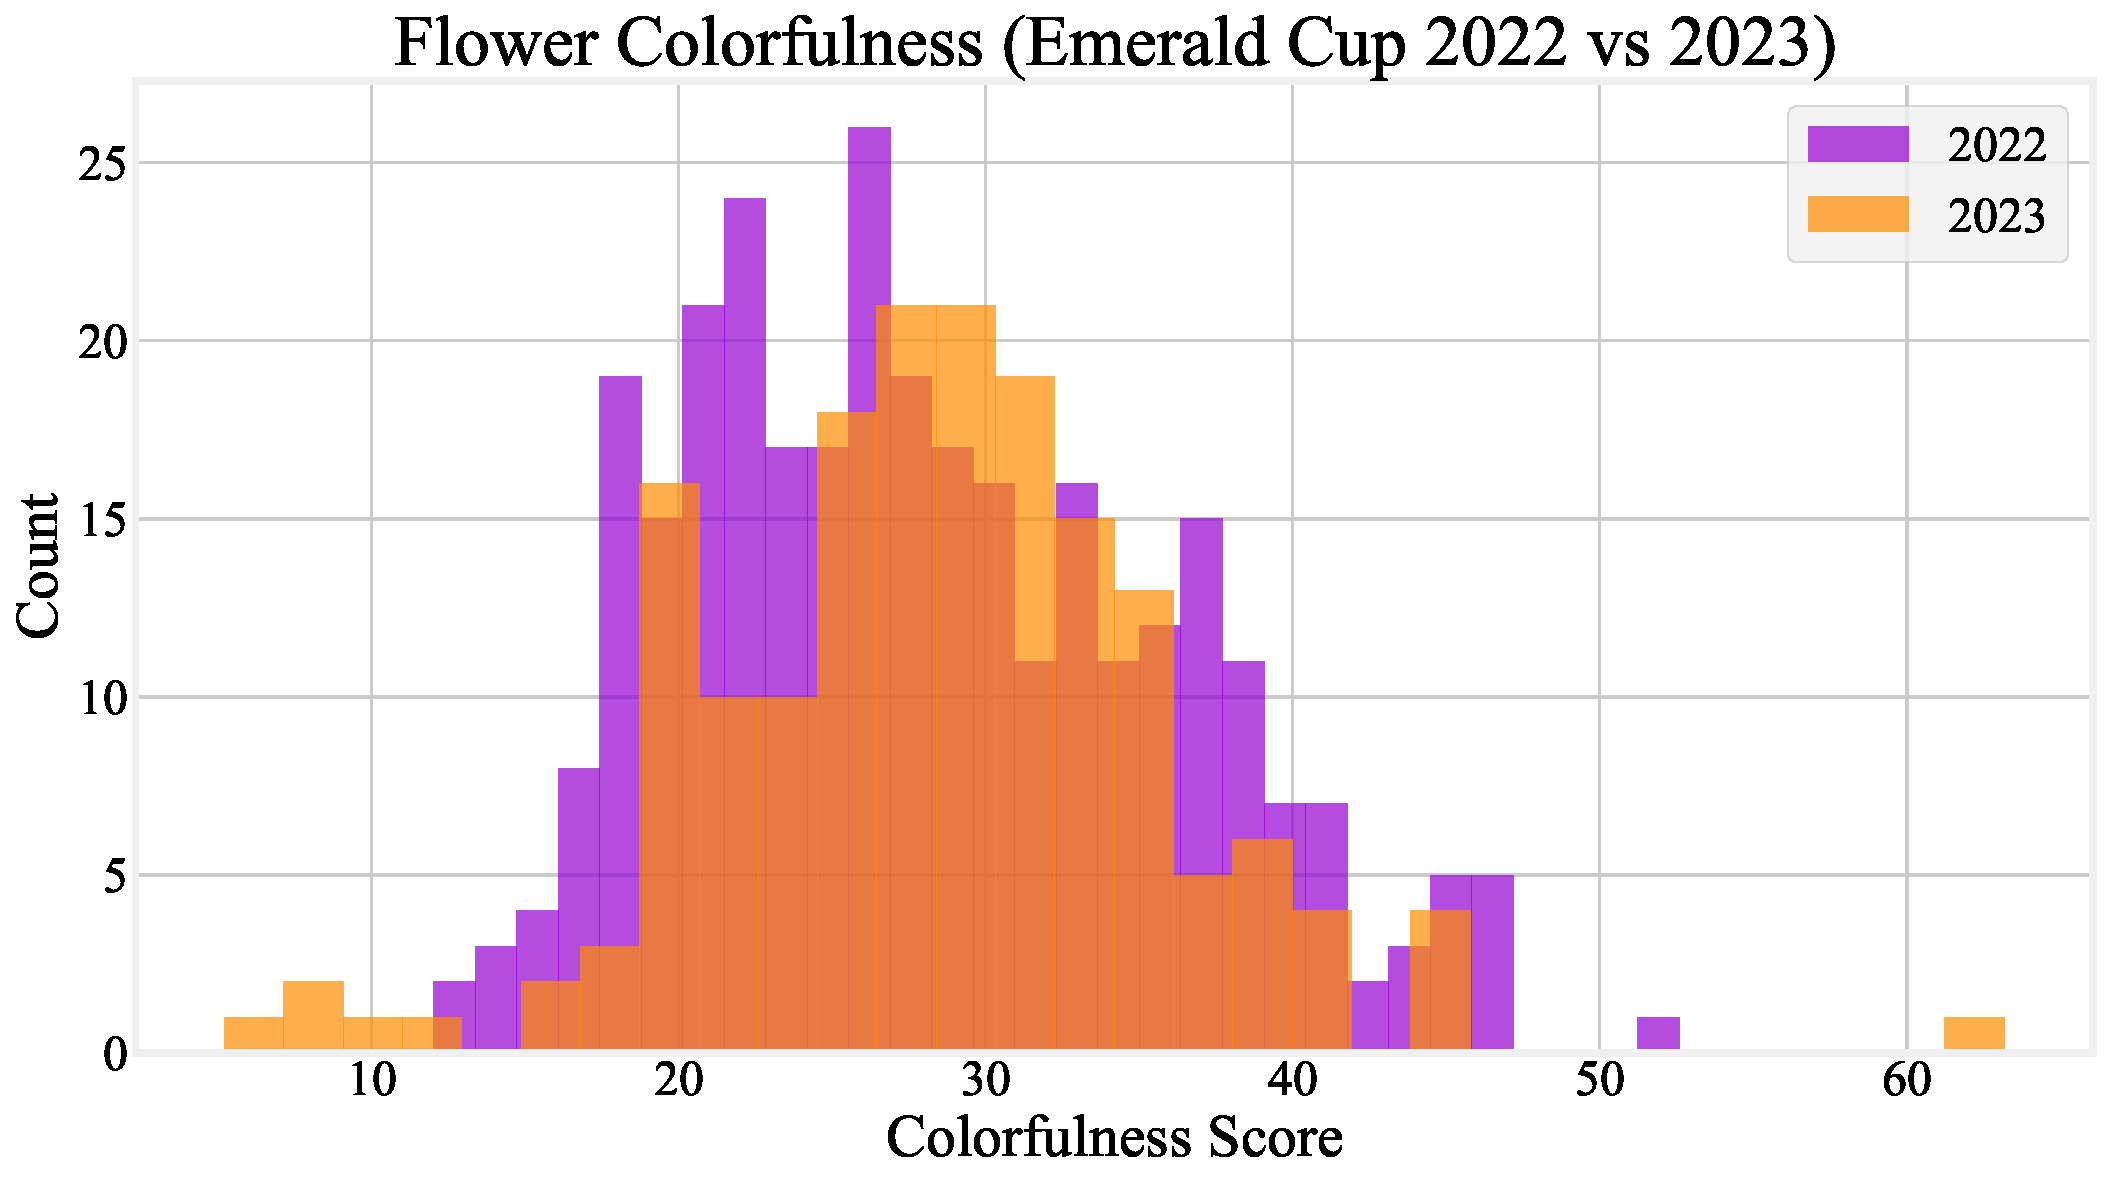
\includegraphics[width=\textwidth]{images/emerald-cup-colorfulness-scores.pdf}
\end{frame}


%------------------------------------------%
% Awards
%------------------------------------------%

\begin{frame}{The Cannlytics Purple Flower Award}

\vspace{\baselineskip}

\textbf{2022 Most Purple Flower}\\
P Silver Squatch - Paula Jobe
\begin{figure}[h]
\centering
\includegraphics[width=0.4\textwidth]{images/silver-squatch.png}
\end{figure}

\textbf{2023 Most Purple Flower}\\
Flow Gardens - Blue Meringue Hemp
\begin{figure}[h]
\centering
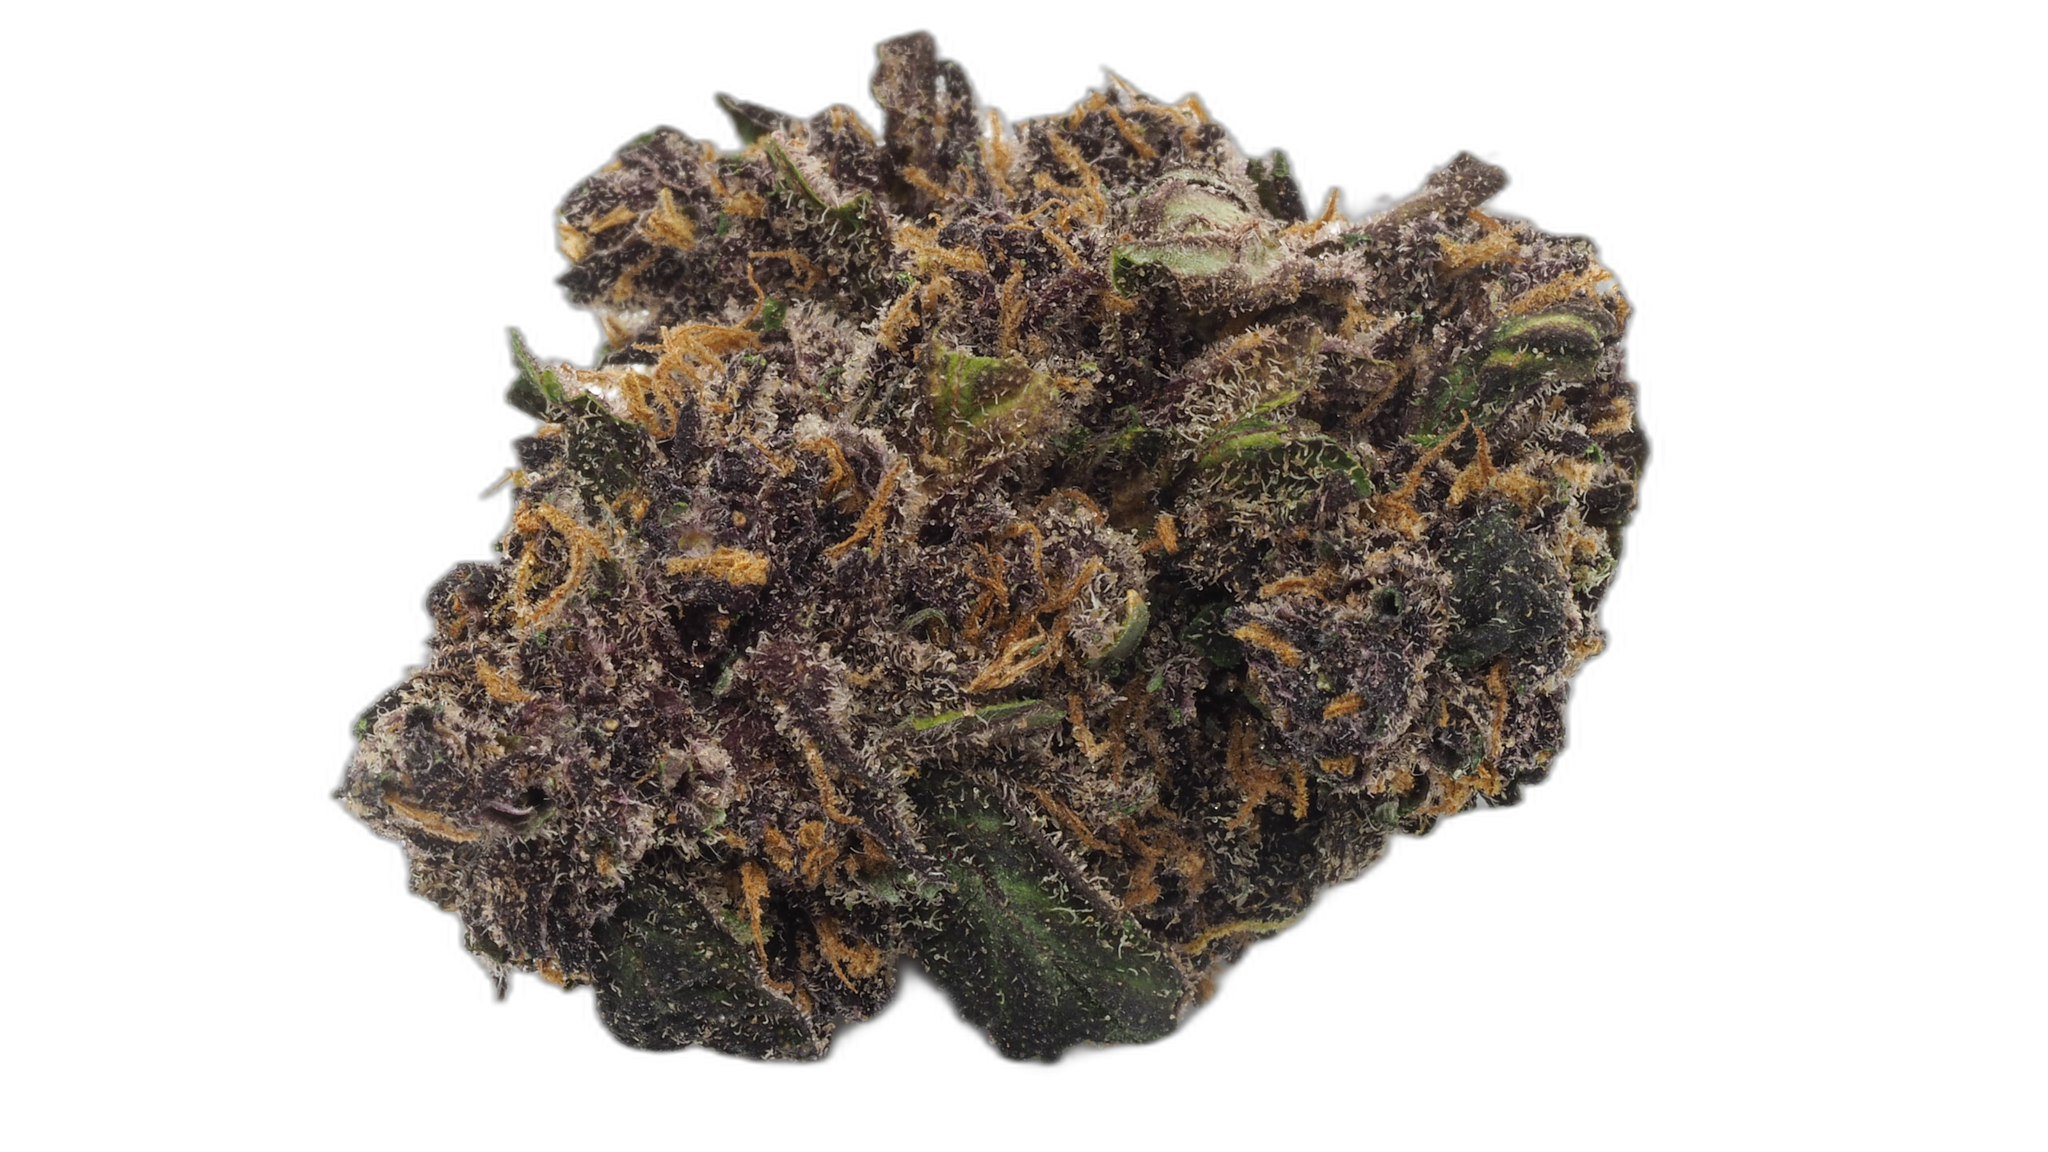
\includegraphics[width=0.4\textwidth]{images/blue-meringue.png}
\end{figure}

\end{frame}


\begin{frame}{The Cannlytics Colorful Flower Award}

\vspace{\baselineskip}

\textbf{2022 Most Colorful Flower}\\
K Rainbow Beltz - Royal Bloodline
\begin{figure}[h]
\centering
\includegraphics[width=0.4\textwidth]{images/rainbow-beltz.png}
\end{figure}

\textbf{2023 Most Colorful Flower}\\
Burr's Place - Orange Creampop 38
\begin{figure}[h]
\centering
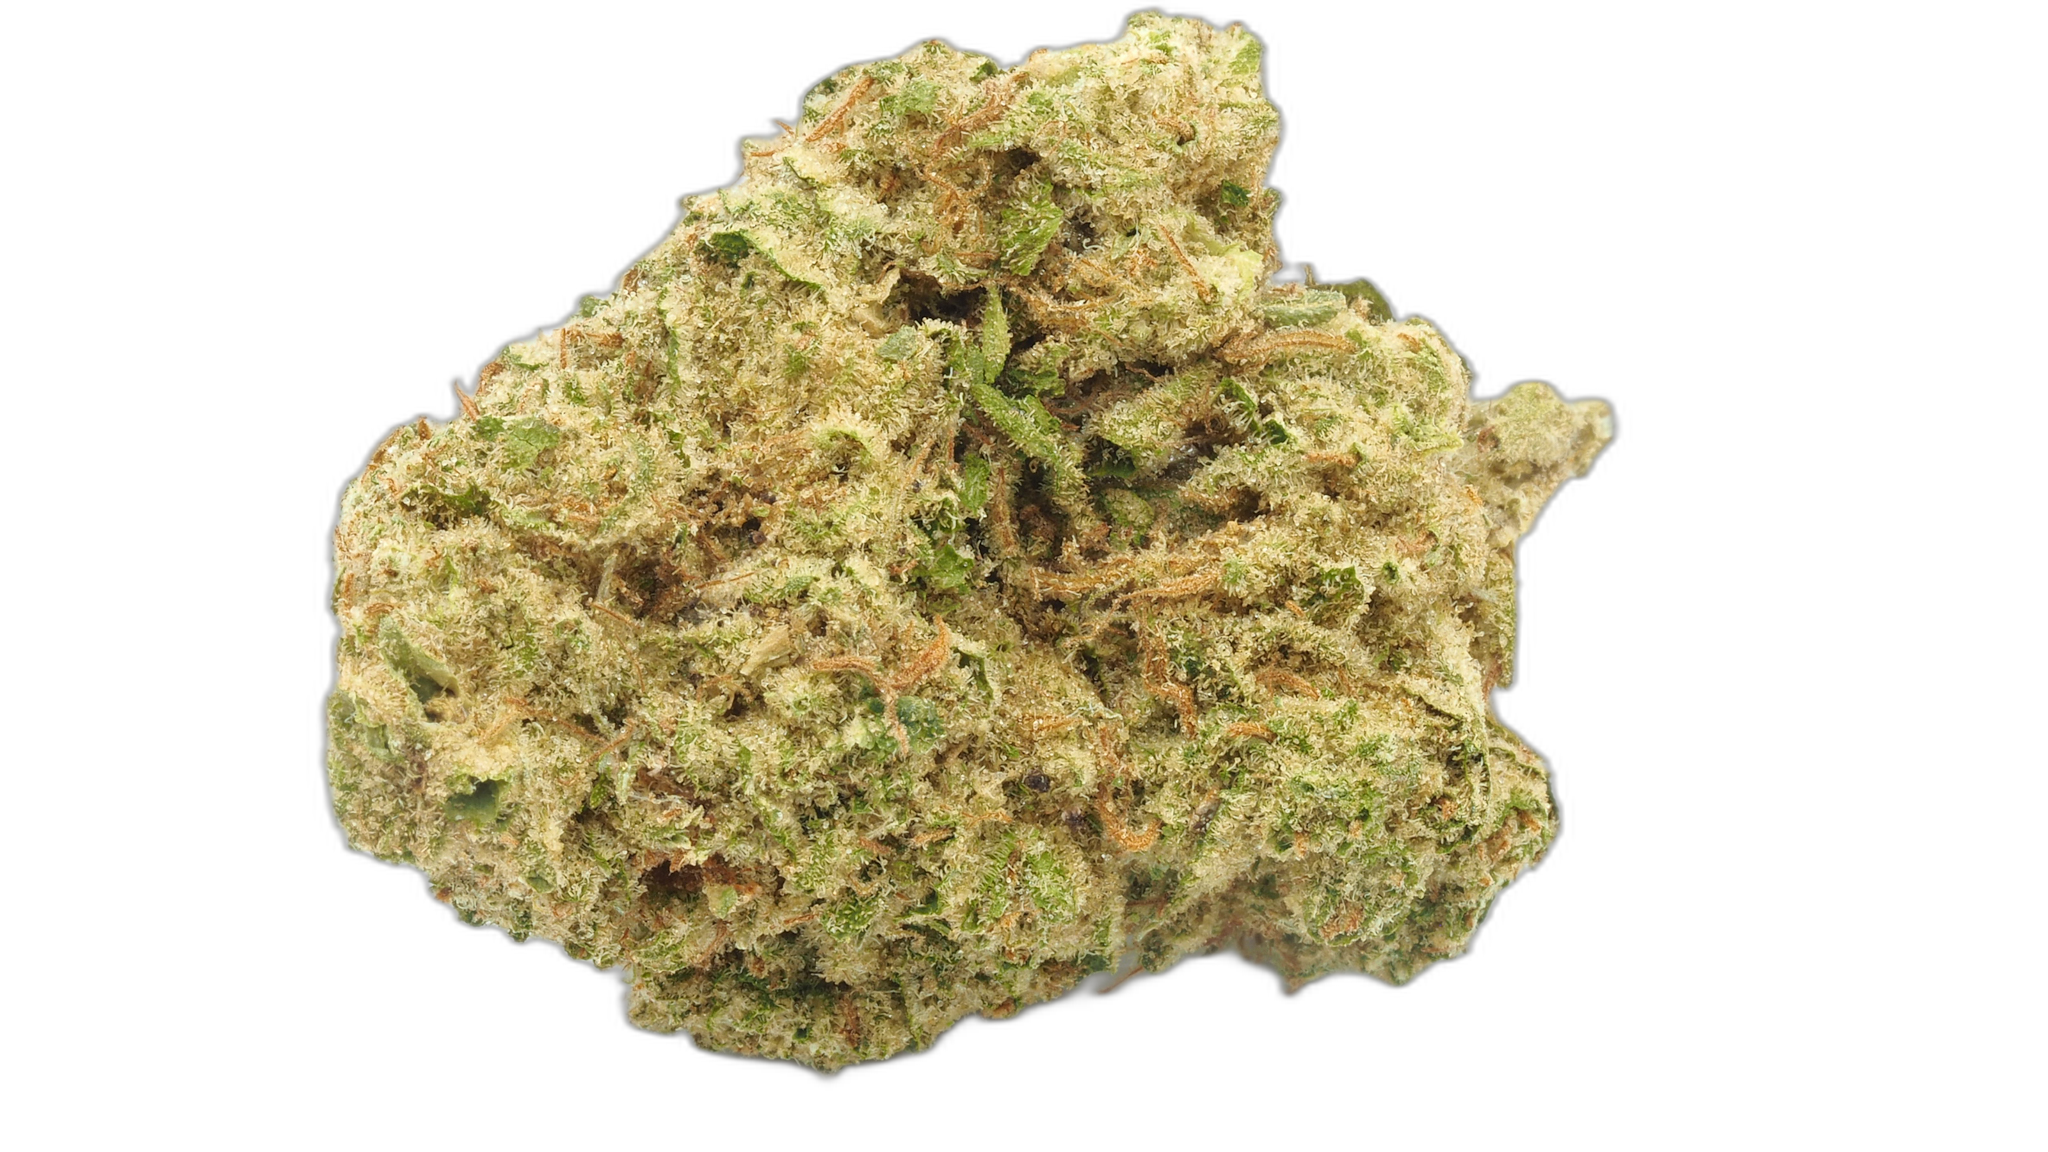
\includegraphics[width=0.4\textwidth]{images/orange-creampop.png}
\end{figure}

\end{frame}

%------------------------------------------%
% Takeaway
%------------------------------------------%
\section{Takeaway}
\begin{frame}{}

\begin{center}
\begin{minipage}{3.85in}

% Thank you.

\includegraphics[width=.25in]{images/prayer.png} {\Large \textbf{Thank you for coming.}}\\

% Re-cap the lesson of the week.
\begin{center}
\begin{minipage}{.9\linewidth}
\begin{Block}{Lessons of the Day}

\vspace{\baselineskip}

\begin{itemize}

\item Sometimes, playing the \textcolor{OliveGreen}{\bfseries waiting game} works so well others don't realize how far ahead you are!

\vspace{\baselineskip}

\end{itemize}

\end{Block}
\end{minipage}
\end{center}

\vfill

\end{minipage}
\end{center}

\end{frame}


%------------------------------------------%
% End
%------------------------------------------%
\end{document}
